% !TeX program = xelatex
\documentclass[11pt]{article}
\usepackage[a4paper,margin=1in]{geometry}
\usepackage{fontspec}
\setmainfont{TeX Gyre Termes}
\usepackage{graphicx}
\usepackage{booktabs}
\usepackage{tabularx}
\usepackage{array}
\usepackage{caption}
\usepackage{float}
\usepackage[section]{placeins}
\usepackage[bottom,hang]{footmisc}
\usepackage{enumitem}
\usepackage{microtype}
\usepackage{hyperref}
\hypersetup{colorlinks=true,linkcolor=black,citecolor=black,urlcolor=blue}
\setlength{\parindent}{0pt}
\setlength{\parskip}{0.55em}
\setcounter{secnumdepth}{2}
\captionsetup{font=small,labelfont=bf}
\pagestyle{empty}

\title{Agent-Based Modeling: Research Trends, LLM Adoption, and Collaboration Networks}
\author{}
\date{A quantitative review of publications, 1972--2025}

\begin{document}
\maketitle
\begin{abstract}
Agent-based modeling (ABM) has developed from a specialized approach to representing heterogeneous interacting entities into a widely used framework for studying coupled social, biological, urban, and technological systems. This review combines a corpus analysis of 29,139 publications from 1972 to 2025 with established research on ABM design, large language model (LLM)-based agents, and scientific collaboration networks. Three findings emerge. First, annual publication output rose from 134 papers in 2000 to 2,495 in 2025, alongside a thematic shift from ecology and the environment toward epidemiology, public health, social dynamics, transport, and urban systems. Second, LLM adoption is measurable but remains at an early stage: the share of ABM papers using LLMs increased from 1.50\% in 2023 to 5.65\% in 2025. Of the identified uses, 59.6\% involved agent behavior or decision-making, while 40.4\% supported implementation, data generation, analysis, or interfaces. Third, collaboration became more extensive and international, yet also more modular: detected communities increased from 8 to 52 across the analyzed periods, with no evidence of general convergence. Together, these findings show how application priorities, agent architectures, and research communities are changing. They also point to a shared agenda: strengthen behavioral validation, transparency, reproducibility, and the evaluation of LLM-enabled agents.

\par\smallskip\noindent\textbf{Keywords:} agent-based modeling; generative agents; large language models; bibliometrics; coauthorship networks; community detection; complex adaptive systems
\end{abstract}

\section{Scope and analytical design}

Agent-based modeling (ABM) explains system-level outcomes through the actions and interactions of heterogeneous agents situated in an environment. Its distinctive contribution is to make the micro-to-macro pathway explicit: agents perceive conditions, follow decision rules, interact within a network or space, and adapt or learn; their interactions can then generate patterns not specified at the aggregate level. ABM is especially useful when heterogeneity, path dependence, feedback, spatial structure, or bounded rationality is central to the research question. \footnote{Bonabeau, E. (2002). Agent-based modeling: Methods and techniques for simulating human systems. Proceedings of the National Academy of Sciences, 99(Suppl. 3), 7280–7287. https://doi.org/10.1073/pnas.082080899; Macal, C. M., \& North, M. J. (2010). Tutorial on agent-based modelling and simulation. Journal of Simulation, 4(3), 151–162. https://doi.org/10.1057/jos.2010.3; Gilbert, N., \& Troitzsch, K. G. (2005). Simulation for the social scientist (2nd ed.). Open University Press; Railsback, S. F., \& Grimm, V. (2019). Agent-based and individual-based modeling: A practical introduction (2nd ed.). Princeton University Press.}

This review draws on a corpus analysis of 29,139 publications dated 1972–2025. Titles and abstracts were classified by application domain, modeled entity, LLM involvement and function, authorship, and country. The analysis combined trend tests, logistic models with Benjamini–Hochberg correction, counterfactual Poisson analyses, and coauthorship community detection. The corpus should therefore be understood as the empirical basis for this review, not as an exhaustive census of every ABM publication. LLM findings in particular are early-diffusion estimates: the post-release observation window covers only 2023–2025. Records were collected from Web of Science, PubMed, and DBLP, deduplicated, and, where possible, enriched with abstracts through OpenAlex. \footnote{Priem, J., Piwowar, H., \& Orr, R. (2022). OpenAlex: A fully-open index of scholarly works, authors, venues, and concepts. arXiv:2205.01833. https://doi.org/10.48550/arXiv.2205.01833} The cleaning workflow excluded records that still lacked abstracts after enrichment, non-research publication types (including editorials, correspondence, and reviews), and non-English publications. The resulting strict corpus contains 29,139 publications through 2025; the broader all-years corpus contains more than 31,000 records. Figure 1 summarizes the collection and filtering process.

Figure 1 distinguishes the all-years record pool from the publication-year cutoff used in the analyses, making the corpus construction and reporting window explicit.

\begin{figure}[htbp]
\centering
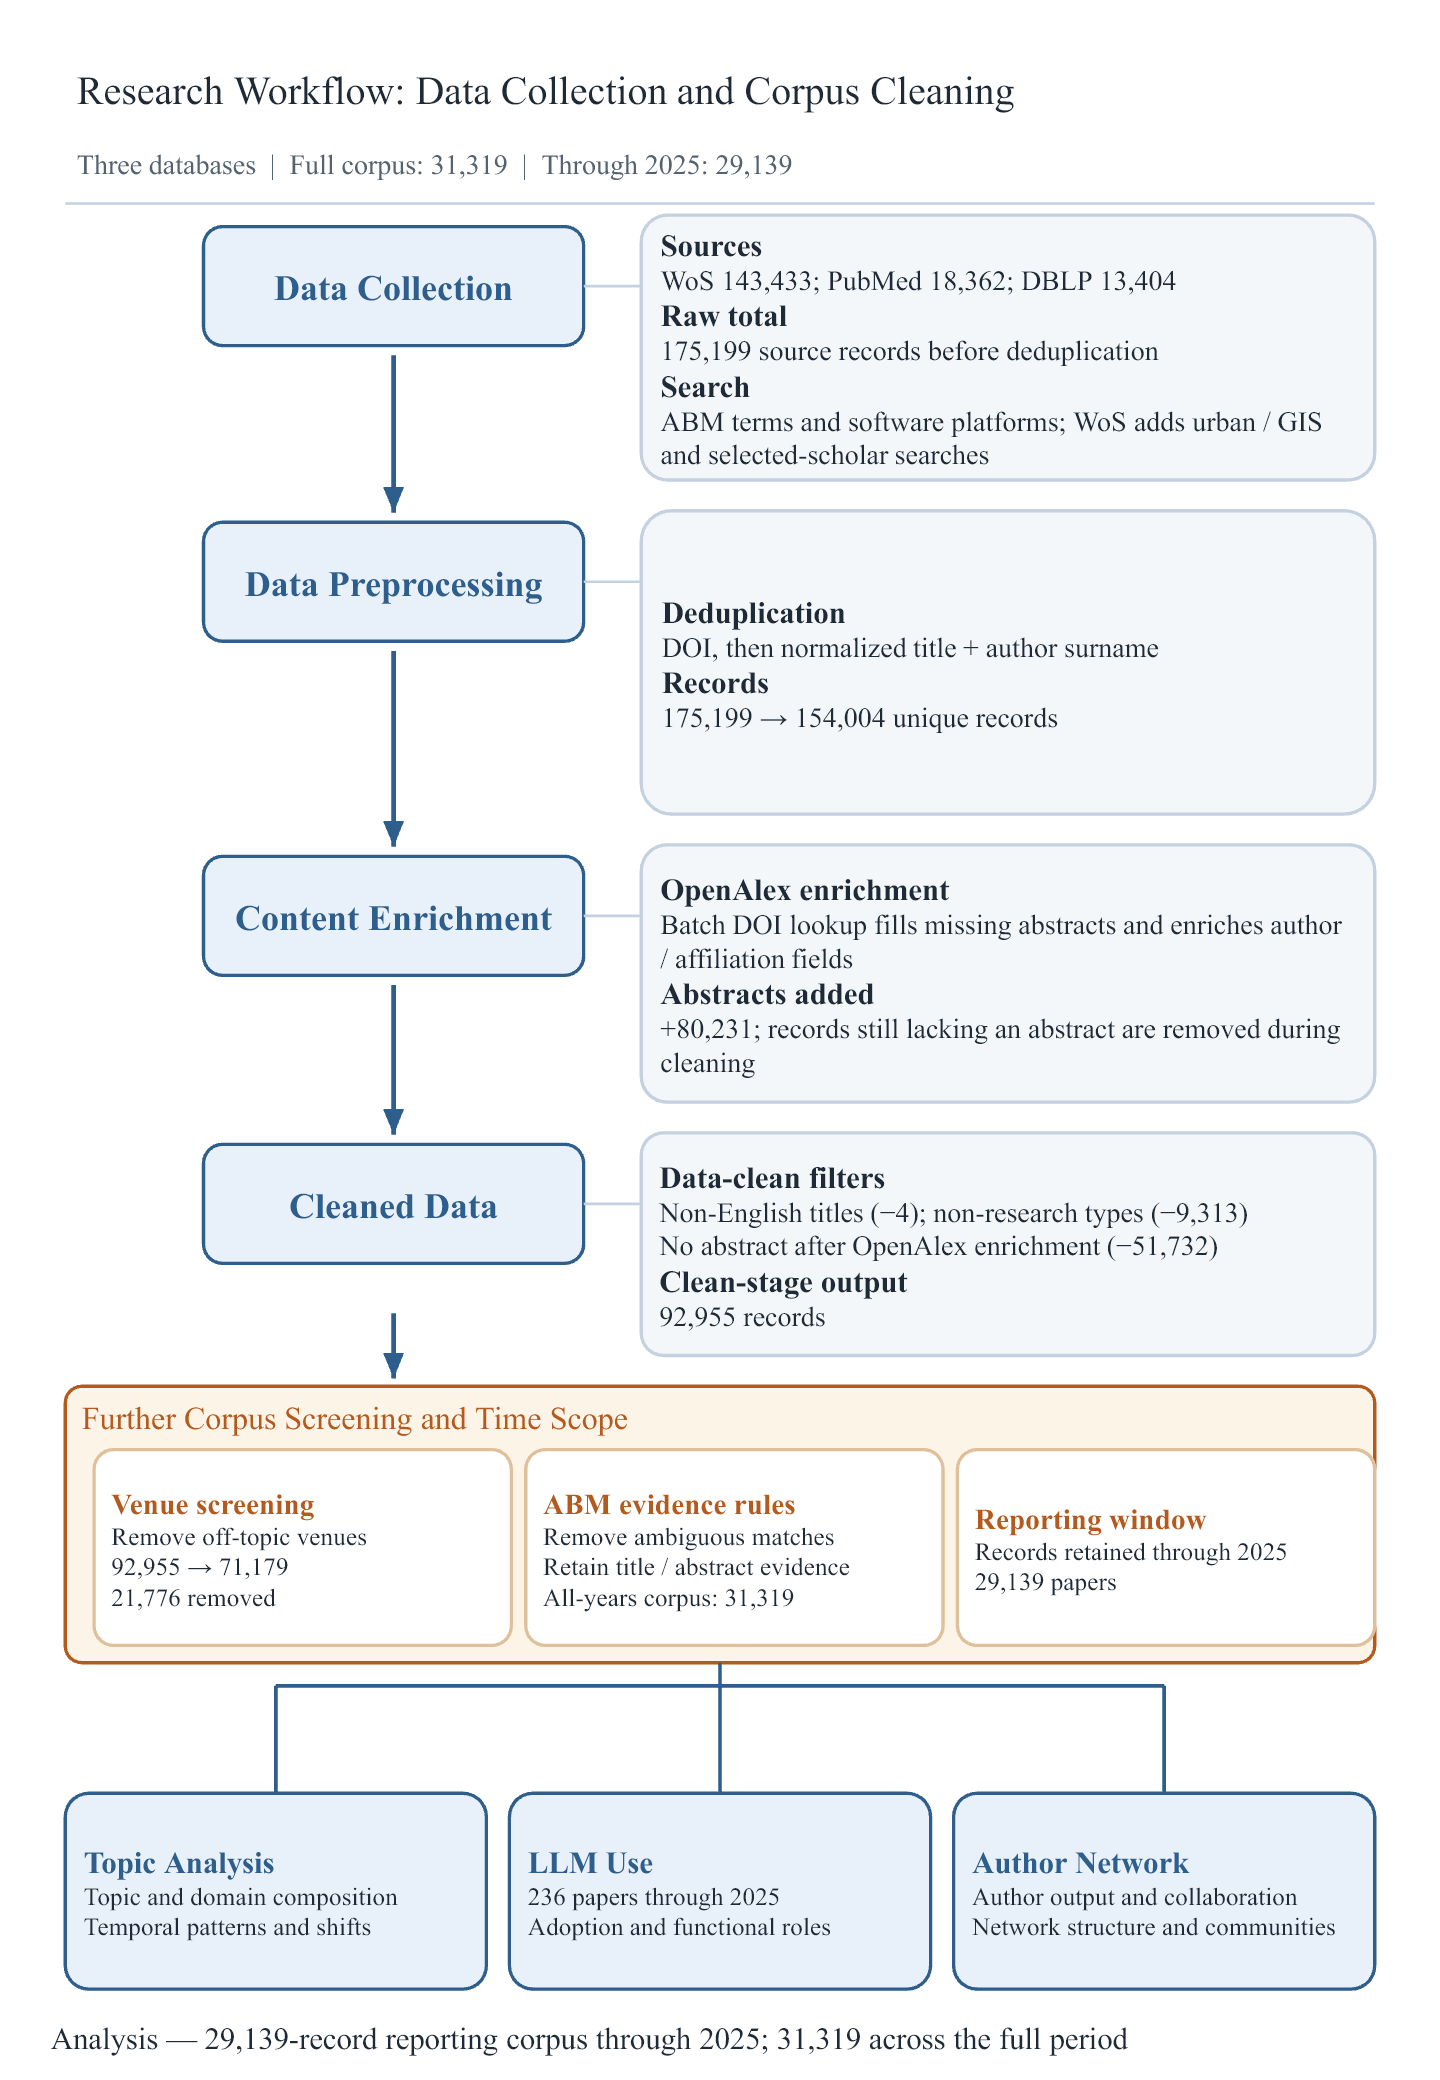
\includegraphics[width=0.88\textwidth,height=0.78\textheight,keepaspectratio]{figures/figure_01.png}
\setcounter{figure}{0}
\caption{Literature collection, abstract enrichment, data cleaning, and derivation of the analytical corpus.}
\label{fig:figure1}
\end{figure}

\begin{table}[htbp]
\centering
\small
\setlength{\tabcolsep}{3pt}
\renewcommand{\arraystretch}{1.18}
\setcounter{table}{0}
\caption{Source of collected papers}
\label{tab:table1}
\begin{tabularx}{\linewidth}{>{\raggedright\arraybackslash}p{0.27\linewidth} >{\centering\arraybackslash}p{0.12\linewidth} X}
\toprule
\textbf{Processing Stage} & \textbf{Number} & \textbf{Description} \\
\midrule
Corpus Collection & 29,139 & — \\
Web of Science & 26,307 & 15,130 papers are indexed exclusively by Web of Science \\
PubMed & 9,671 & 607 papers are indexed exclusively by PubMed \\
DBLP & 4,640 & 2,201 papers are indexed exclusively by DBLP \\
Overlapping Records Across Databases & 11,201 & Papers indexed by two or more databases; therefore, the sum of database-specific counts exceeds the total corpus size \\
Papers Using Large Language Models & 236 & As of 2025 \\
\bottomrule
\end{tabularx}
\end{table}

\subsection{DeepSeek API classification and prompt design}

Corpus-level classification used the DeepSeek API through an OpenAI-compatible asynchronous client and the deepseek-chat model. Each request included a paper’s title and abstract; abstracts were truncated at 6,000 characters, and records without an abstract were not submitted for classification. Requests used temperature 0, JSON-object output, and a 512-token response limit. The asynchronous run used checkpoints and retried eligible failures, allowing processing to resume without replacing completed results.

The classification prompt was structured as follows:

\begin{itemize}[leftmargin=1.6em,itemsep=2pt,topsep=3pt]

\item \textbf{Role:} Act as a classifier of literature on agent-based modeling (ABM) and complex systems.

\item \textbf{Evidence:} Use only information stated in the title and abstract; do not infer unsupported details.

\item \textbf{Classification fields:} Assign one primary topic, one dominant simulated-agent type, whether an LLM is used, and—if applicable—the LLM’s functional role, using the supplied standardized taxonomies.

\item \textbf{LLM-use criteria:} Count LLM use only when the model contributes to the research method. Do not count background mentions or use limited to writing, editing, translation, or literature searching. Do not treat conventional machine-learning or NLP methods as LLMs by default.

\item \textbf{Agent-type distinction:} Assign the LLM-agent category only when an LLM is part of the simulated agent architecture; distinguish this from using an LLM to support other research tasks.

\item \textbf{Output format:} Return a compact JSON object with the specified fields and taxonomy codes, without additional prose or formatting.

\end{itemize}

The returned JSON was parsed and checked before being merged with the corpus. This constrained design improves consistency and auditability, but it does not remove classification uncertainty or the need for human validation.
\section{Research trends in agent-based modeling}

\subsection{From methodological niche to cross-domain infrastructure}

\begin{figure}[htbp]
\centering
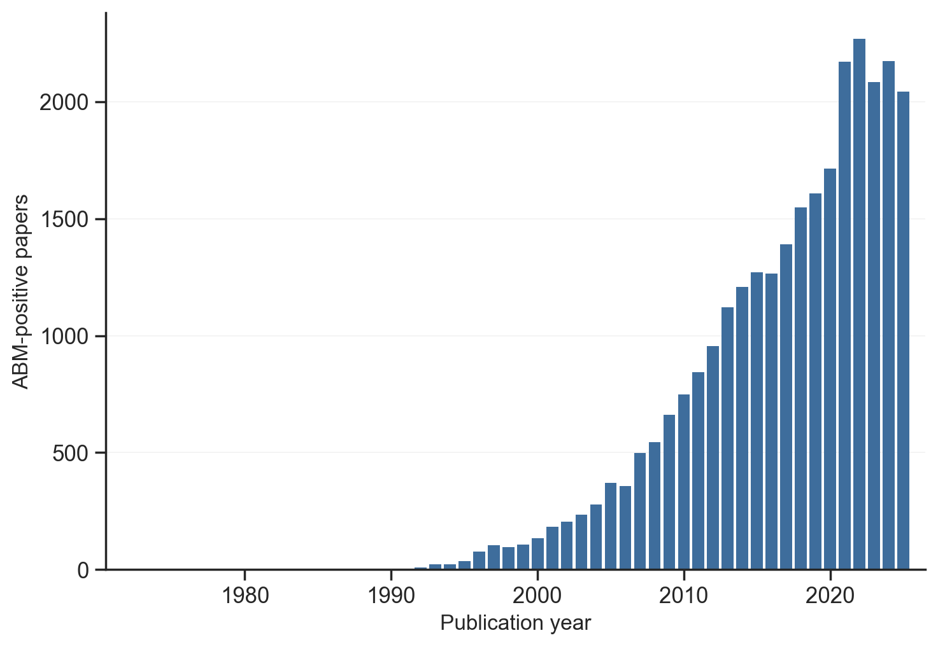
\includegraphics[width=0.96\textwidth,height=0.78\textheight,keepaspectratio]{figures/figure_02.png}
\setcounter{figure}{1}
\caption{Annual publication counts for the strict ABM corpus, 1972–2025 (n = 29,139).}
\label{fig:figure2}
\end{figure}

ABM research expanded steadily and diversified across disciplines. The corpus grew approximately nineteen-fold between 2000 and 2025, marking a shift from a specialized simulation approach to a framework used across many research areas. The increase was not a single abrupt departure from the previous trend. A segmented Poisson model identified 2021 as a potential breakpoint and estimated a 24.0\% increase in publication intensity (z = 6.36, p = 2.0 × 10−10). Yet observed output in 2021–2023 (3,774 papers) was close to the pre-breakpoint projection (3,945 papers), with no significant excess (rate ratio = 0.957, p = 0.997). After adjustment for overall retrieval trends, the estimated change associated with this high-growth period was also not significant (−1.8\%, p = 0.846).

Taken together, the analyses are more consistent with cumulative diffusion across scientific domains than with a single external shock. Publication growth alone, however, cannot show how the field itself changed. The next sections therefore examine domain composition and thematic shifts, separating expansion in the number of papers from redistribution of attention across research areas.

\subsection{Thematic reorientation}

The corpus spans a broad range of applications, although a few domains account for much of the research. Epidemiology and public health is the largest identified domain (7,271 papers; 24.95\%), followed by simulation methodology (4,986; 17.11\%) and ecology and environment (4,564; 15.66\%). The two leading application domains—epidemiology/public health and ecology/environment—together represent 40.62\% of the corpus. Transport (9.79\%), social and opinion dynamics (8.53\%), and urban and land-use systems (6.70\%) form a second tier. This distribution is consistent with ABM’s value for studying interactions among heterogeneous entities and their aggregate consequences. The substantial methodology category also shows that growth includes continued work on ABM itself, not applications alone.

\begin{figure}[htbp]
\centering
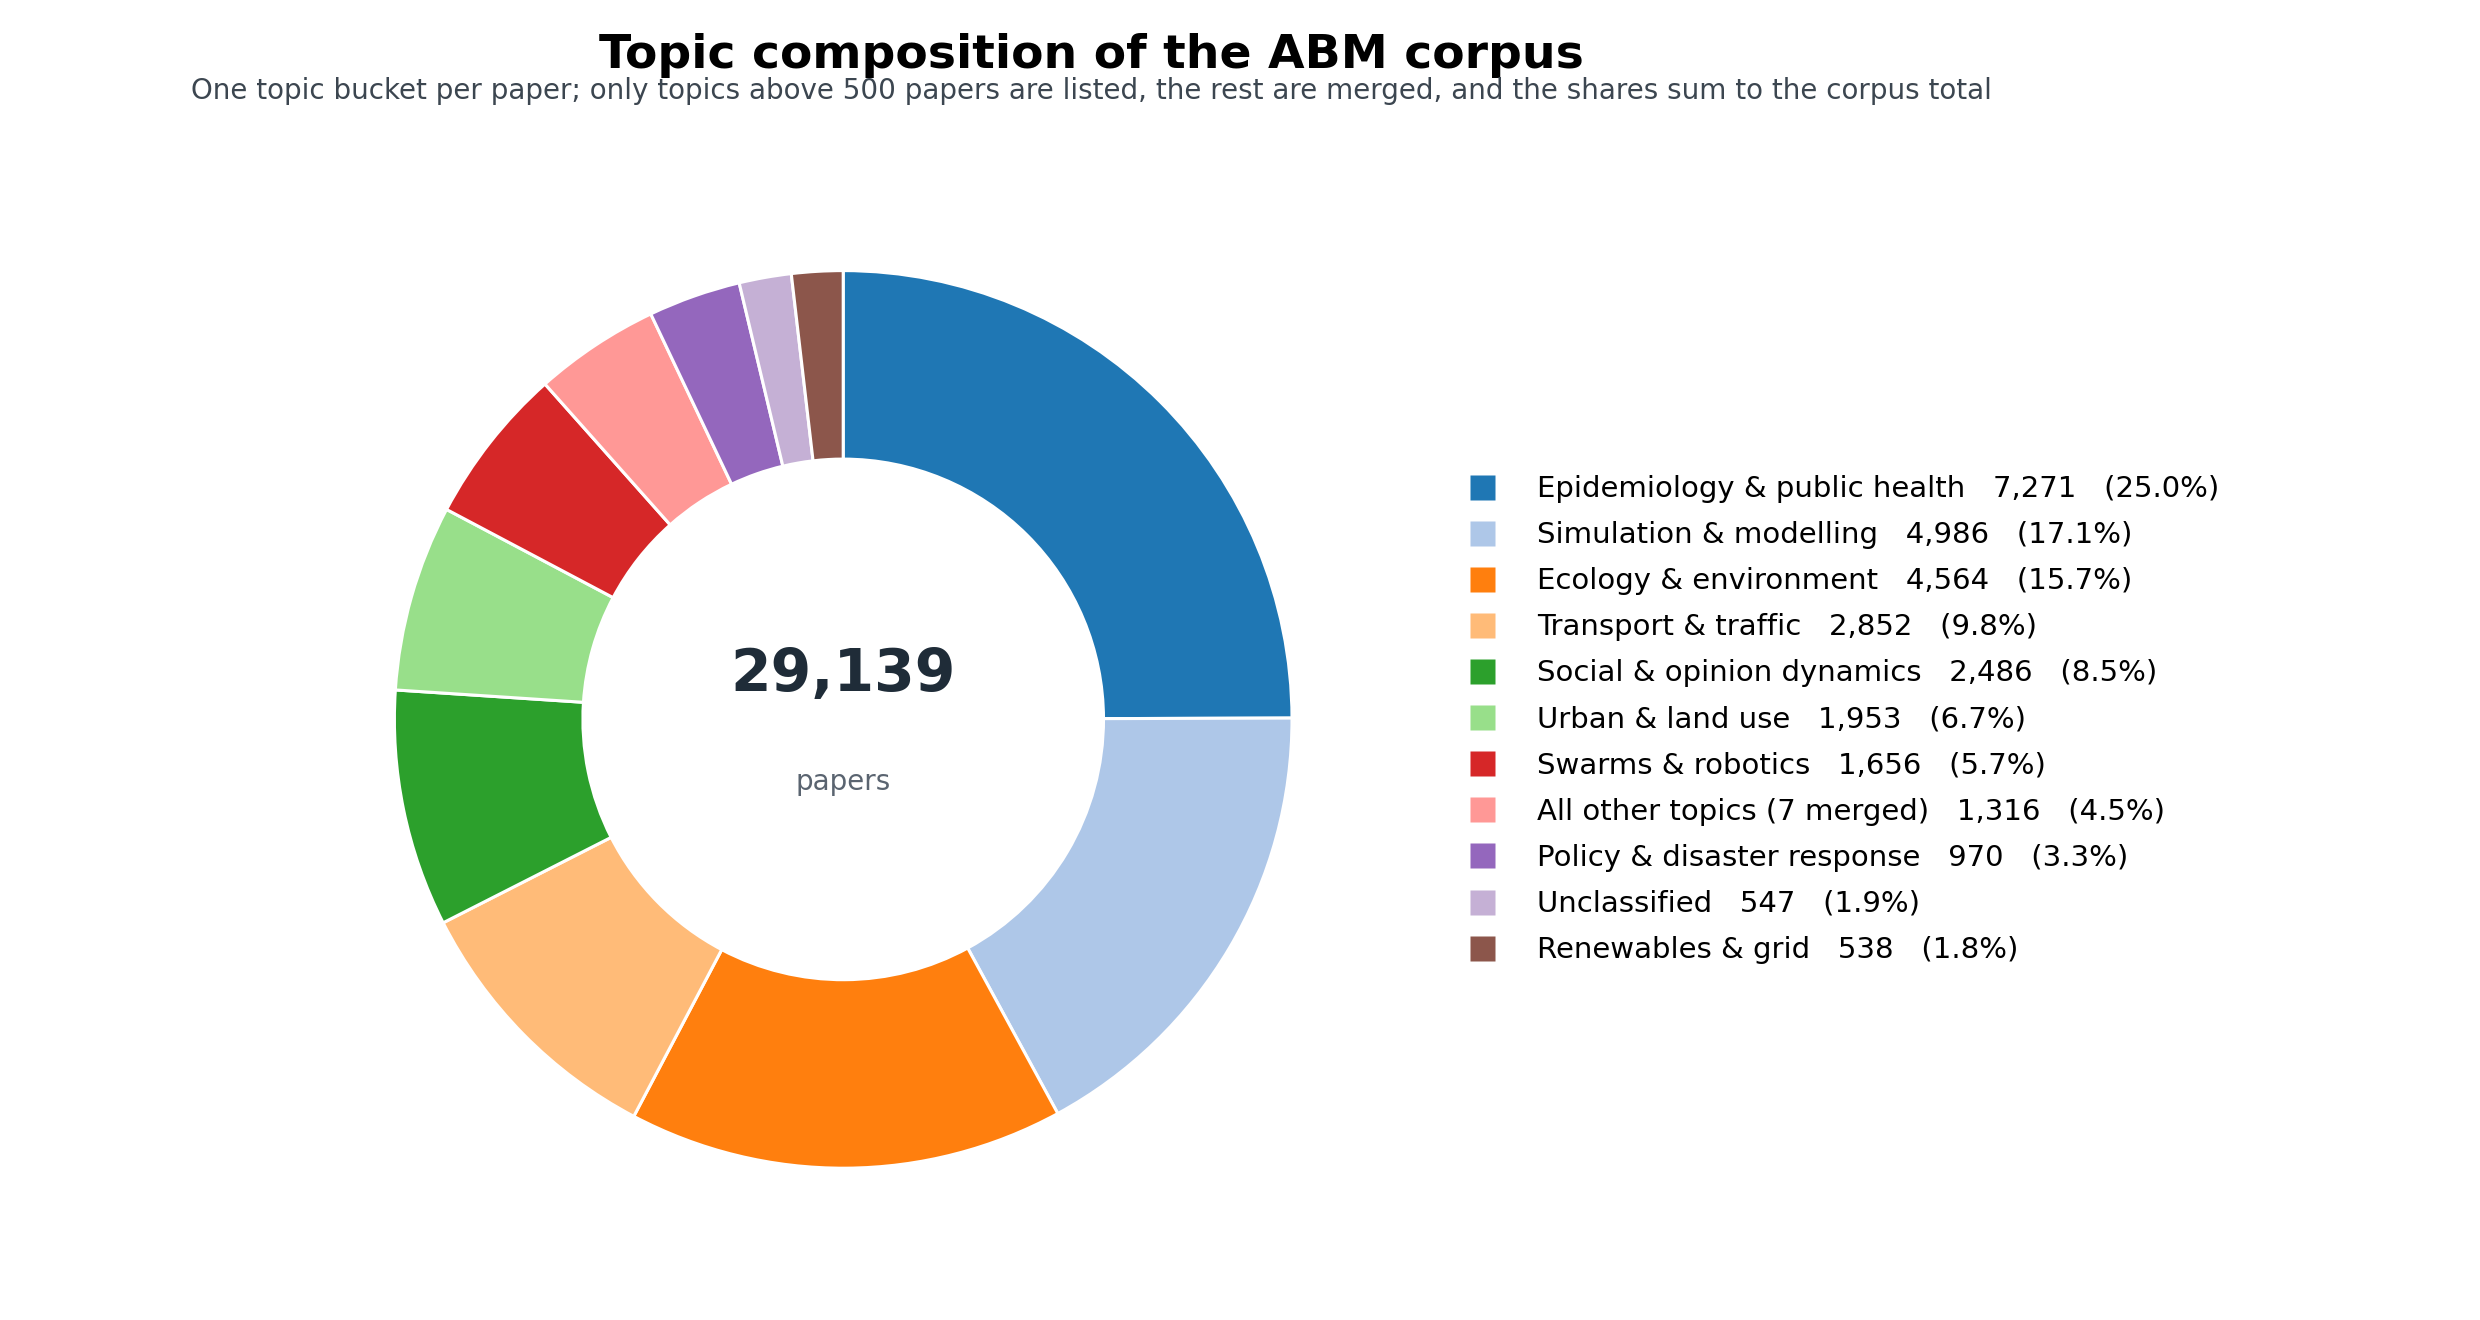
\includegraphics[width=0.96\textwidth,height=0.78\textheight,keepaspectratio]{figures/figure_03.png}
\setcounter{figure}{2}
\caption{Overall thematic composition of the ABM corpus.}
\label{fig:figure3}
\end{figure}

The annual series shows that the field’s composition changed alongside its overall growth. Ecology and environment declined from about 28.0\% of papers in 2001 to roughly 15\% in 2025. Epidemiology and public health rose from about 15.3\% in 2001, peaked at 40.9\% in 2022, and remained the leading application family through 2025. Transport also gained share—from roughly 2–3\% around 2000 to about 11\% in 2025—while social and opinion dynamics became an established line of work. These changes indicate a broader portfolio in which human behavior, institutions, mobility, communication, and policy are studied alongside environmental processes; they do not mean that earlier areas have disappeared.

\begin{figure}[htbp]
\centering
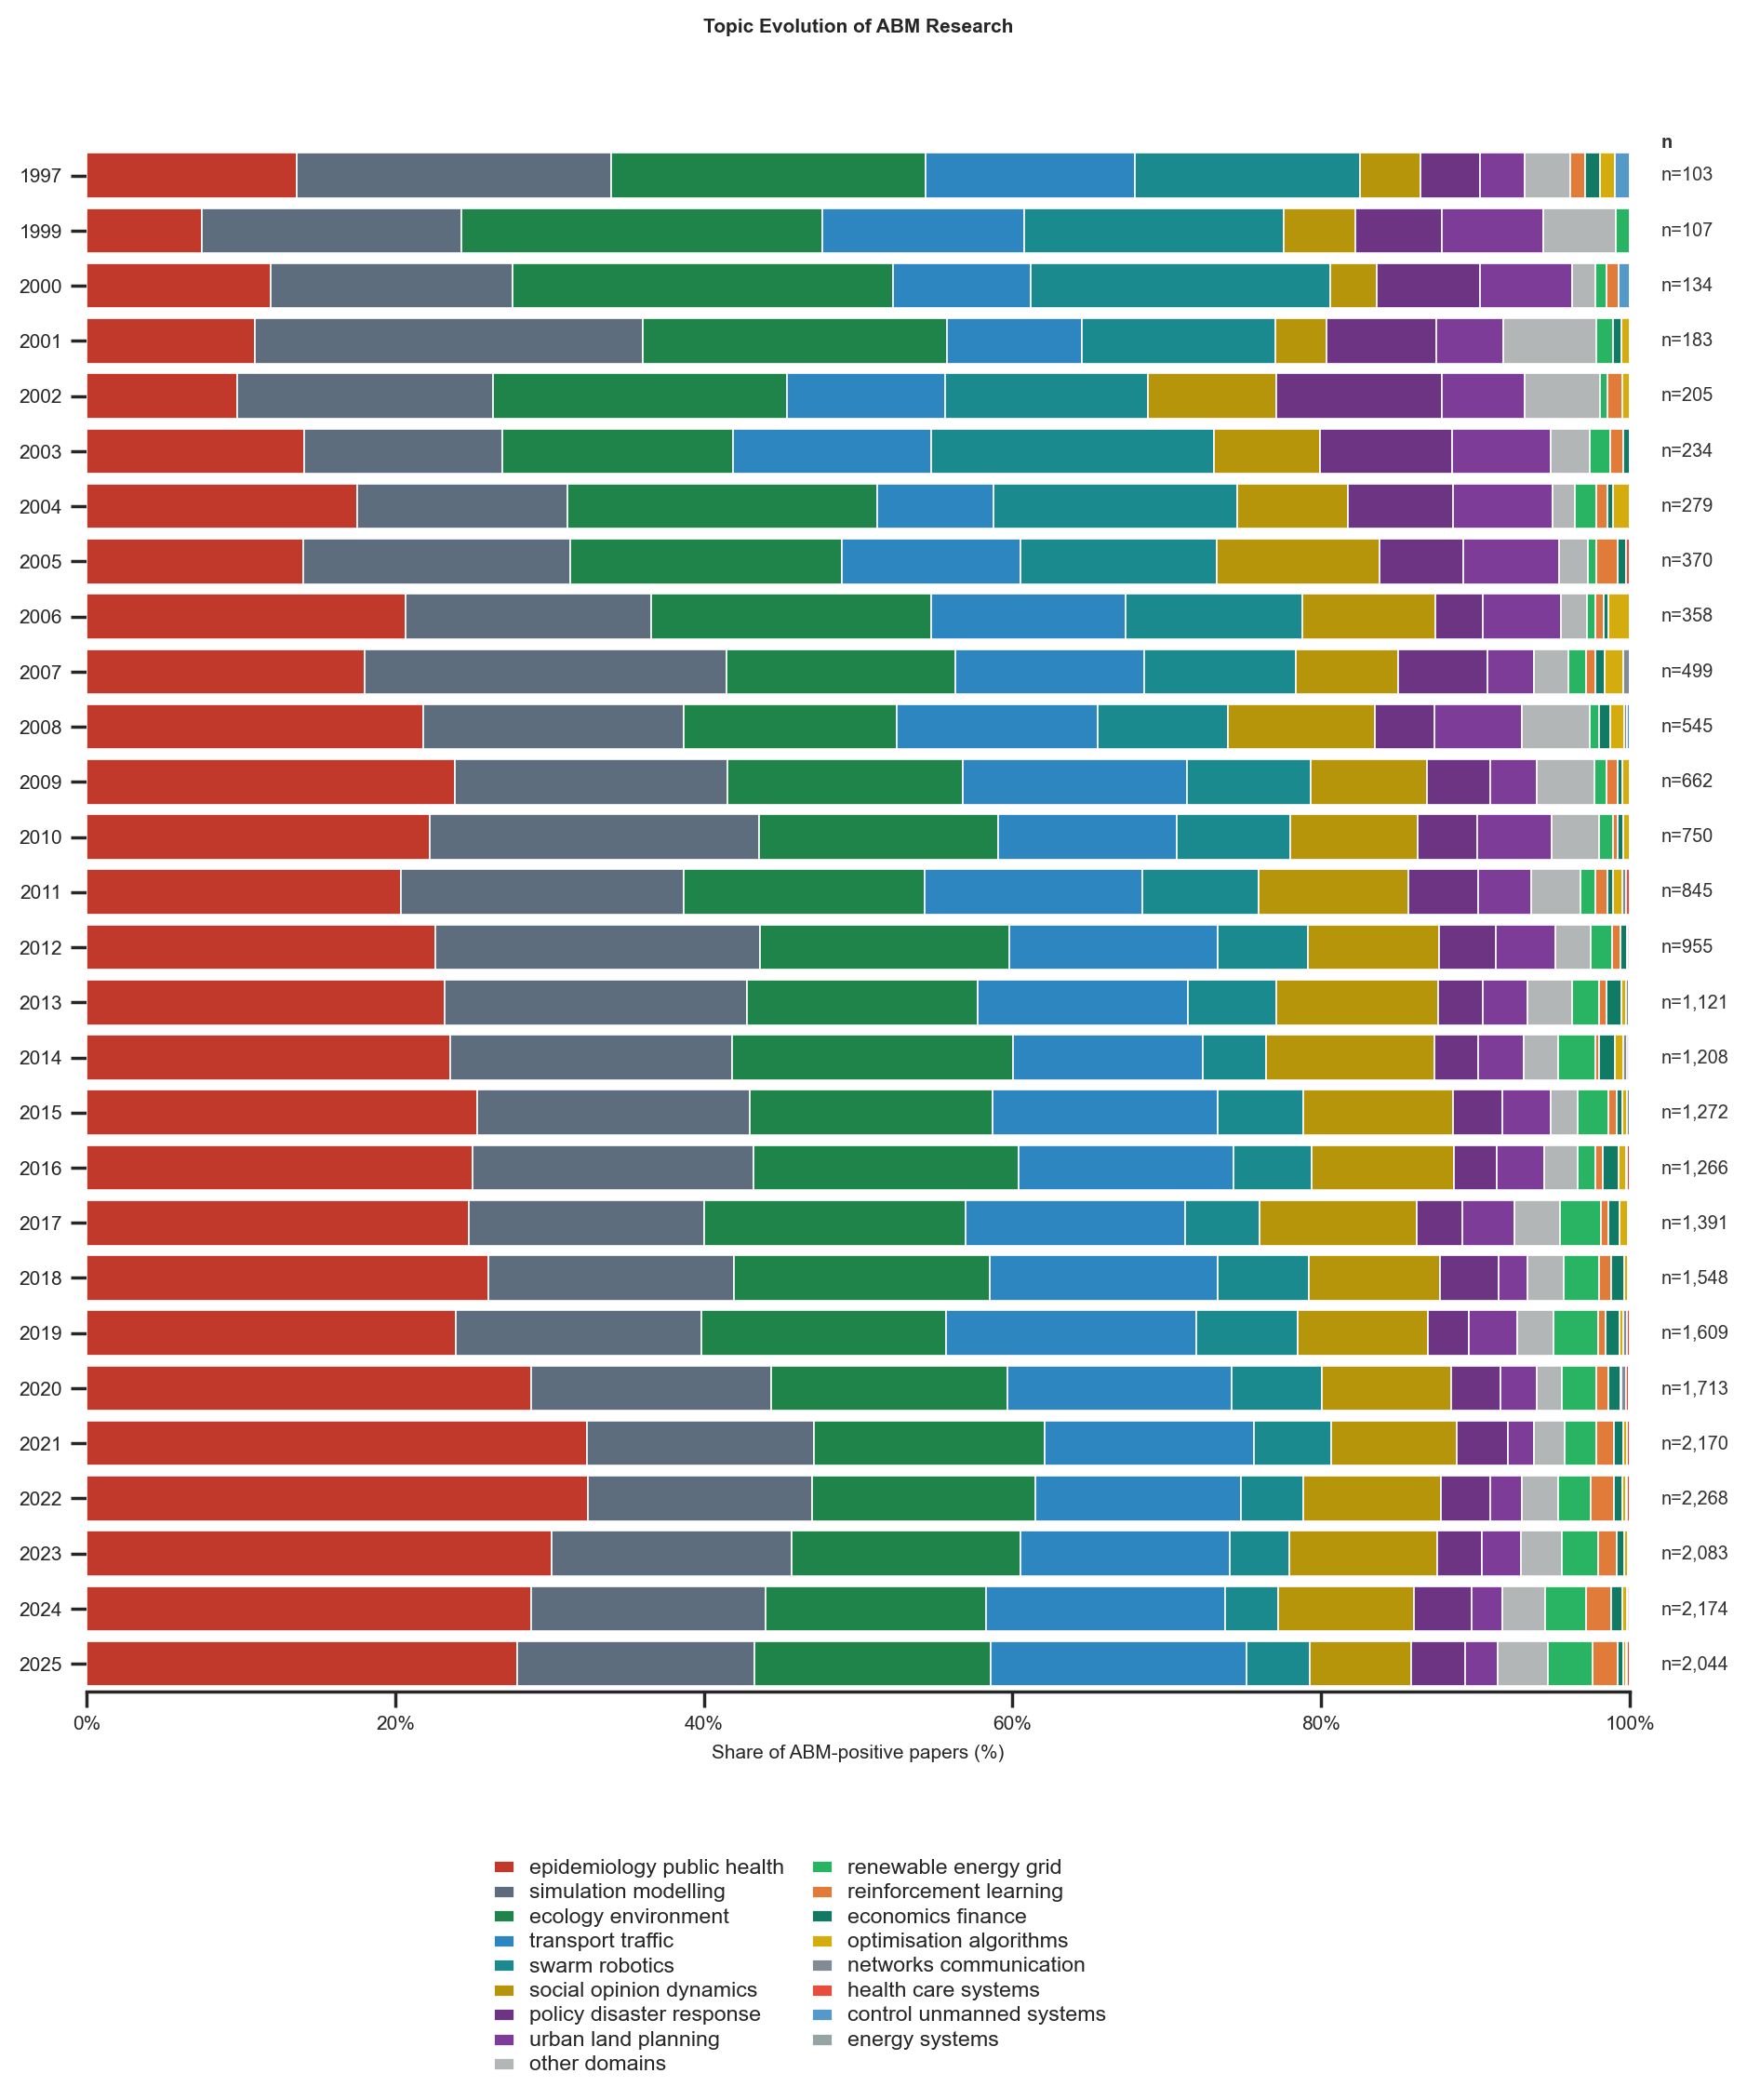
\includegraphics[width=0.96\textwidth,height=0.78\textheight,keepaspectratio]{figures/figure_04.png}
\setcounter{figure}{3}
\caption{Annual evolution of thematic composition, 2001–2025.}
\label{fig:figure4}
\end{figure}

\begin{figure}[htbp]
\centering
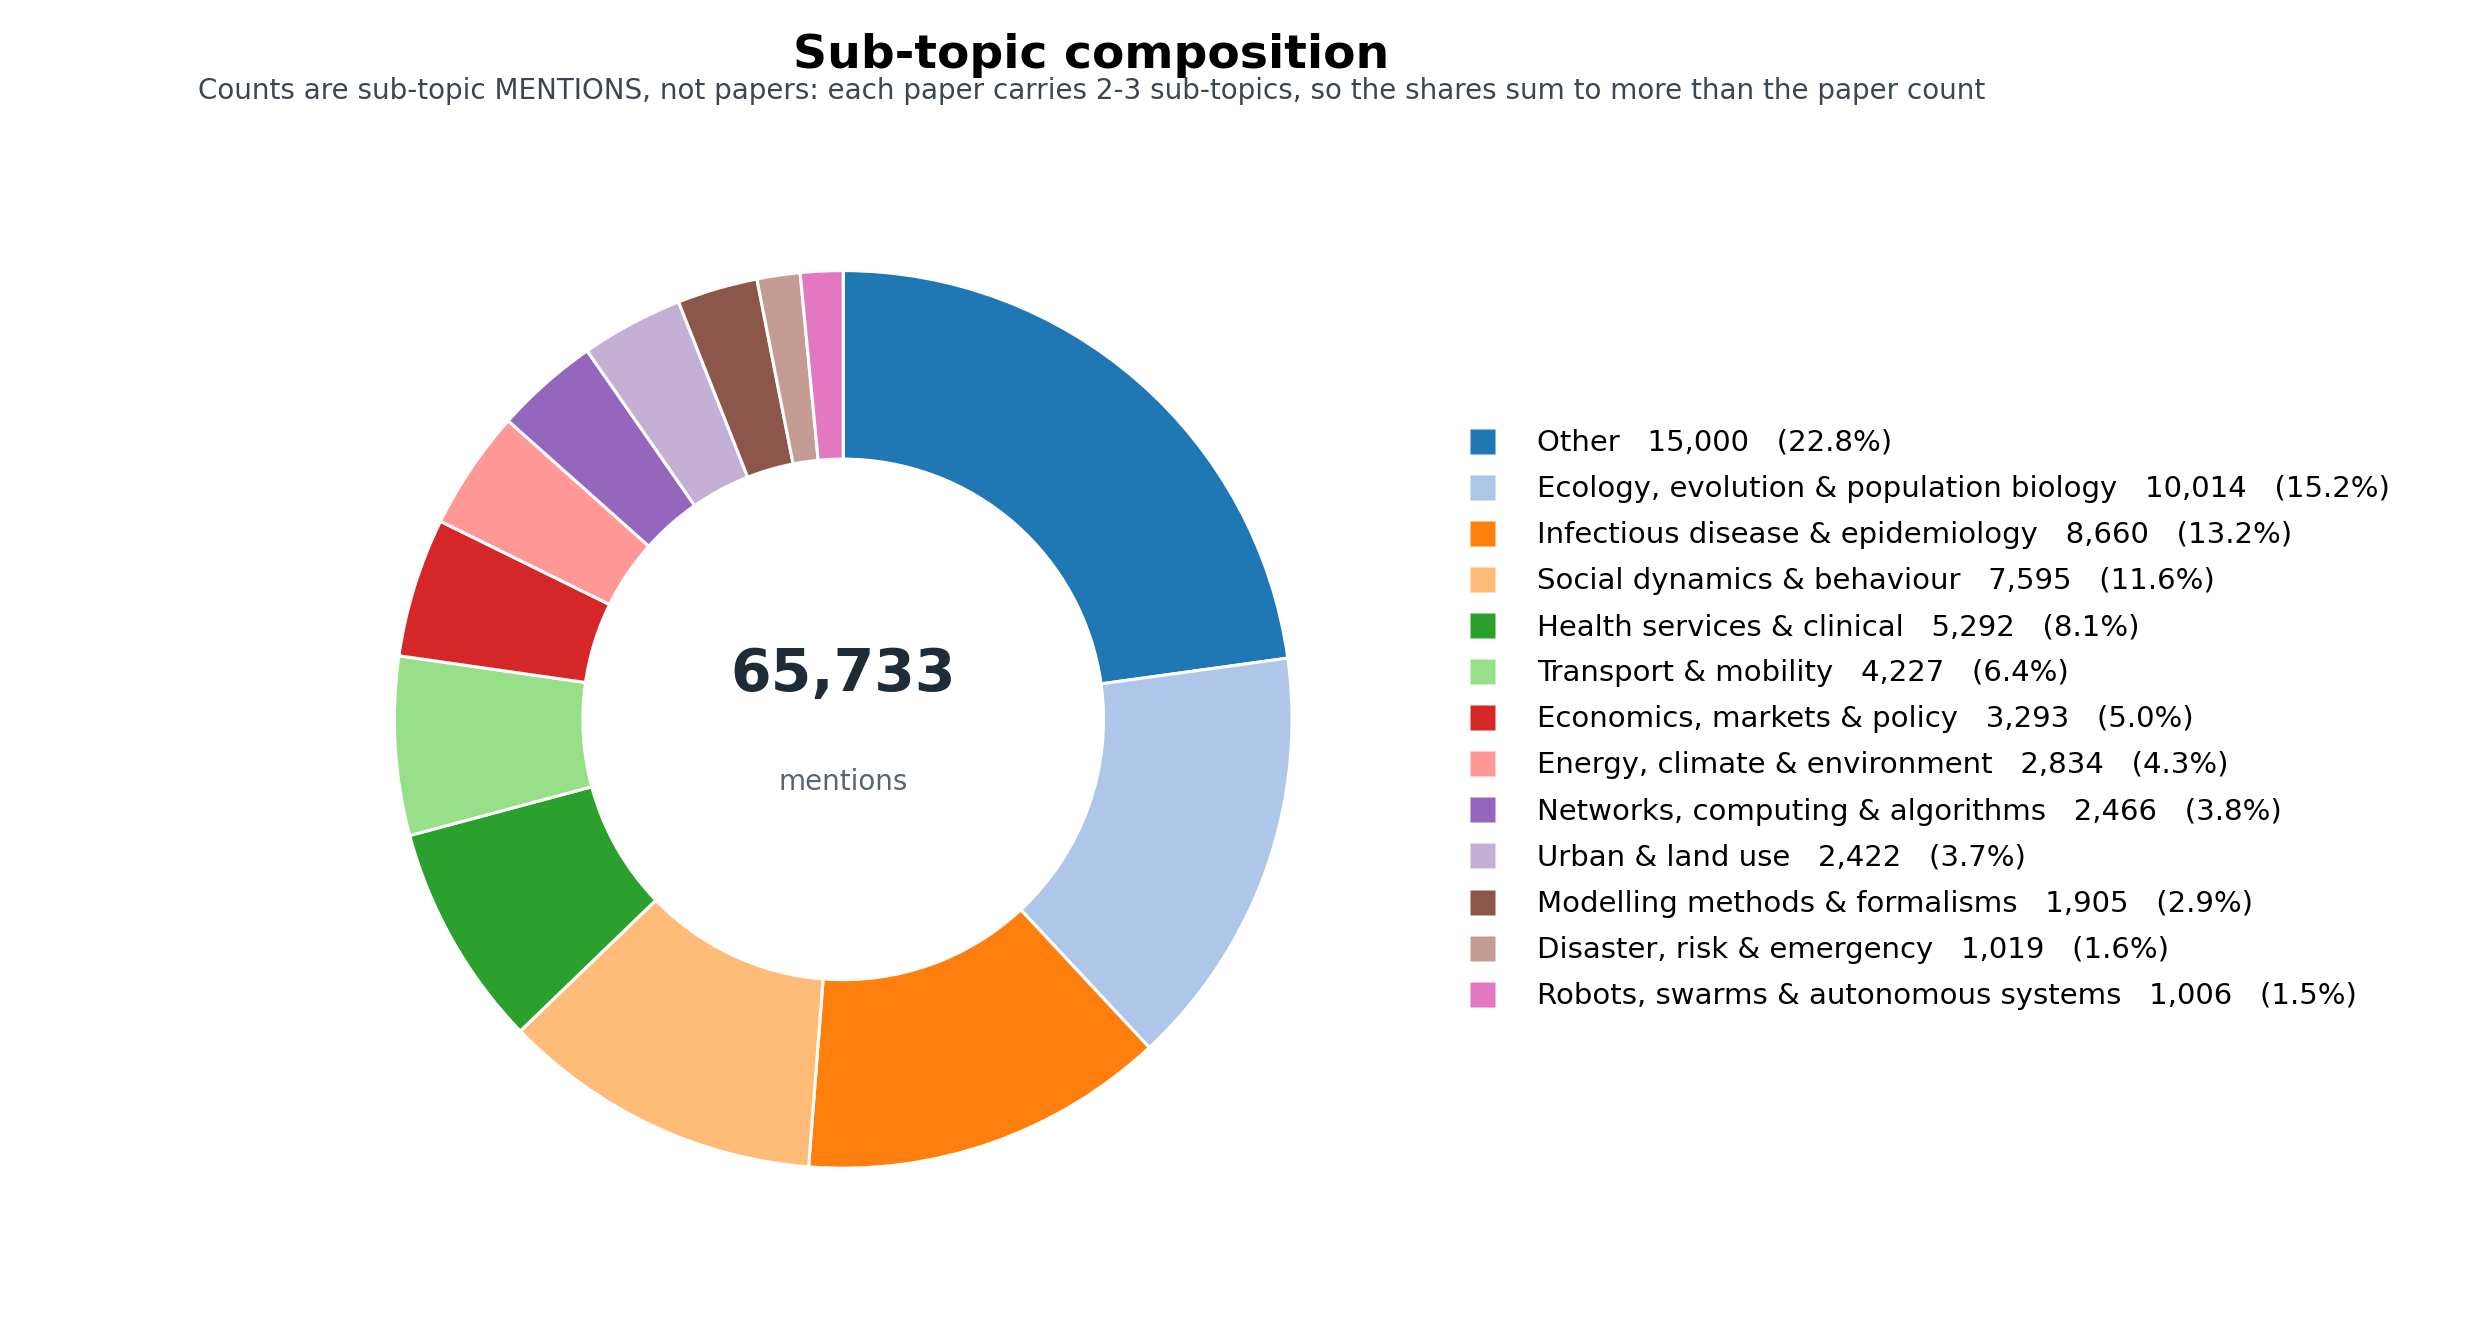
\includegraphics[width=0.96\textwidth,height=0.78\textheight,keepaspectratio]{figures/figure_05.png}
\setcounter{figure}{4}
\caption{Subtheme composition of the corpus.}
\label{fig:figure5}
\end{figure}

Subthemes reveal more detail within the broad domains (Figure 5). Ecology, evolution, and population biology account for 10,014 mentions (15.2\%), followed by infectious disease and epidemiology (8,660; 13.2\%) and social dynamics and behaviour (7,595; 11.6\%). Health services and clinical research (8.1\%) and transport and mobility (6.4\%) are also prominent. These are subtheme mentions, not unique papers: each paper can receive two or three labels. The 65,733 total mentions therefore exceed the corpus size, and percentages represent shares of assigned mentions. “Other” combines less frequent subthemes rather than denoting one substantive topic.

\begin{figure}[htbp]
\centering
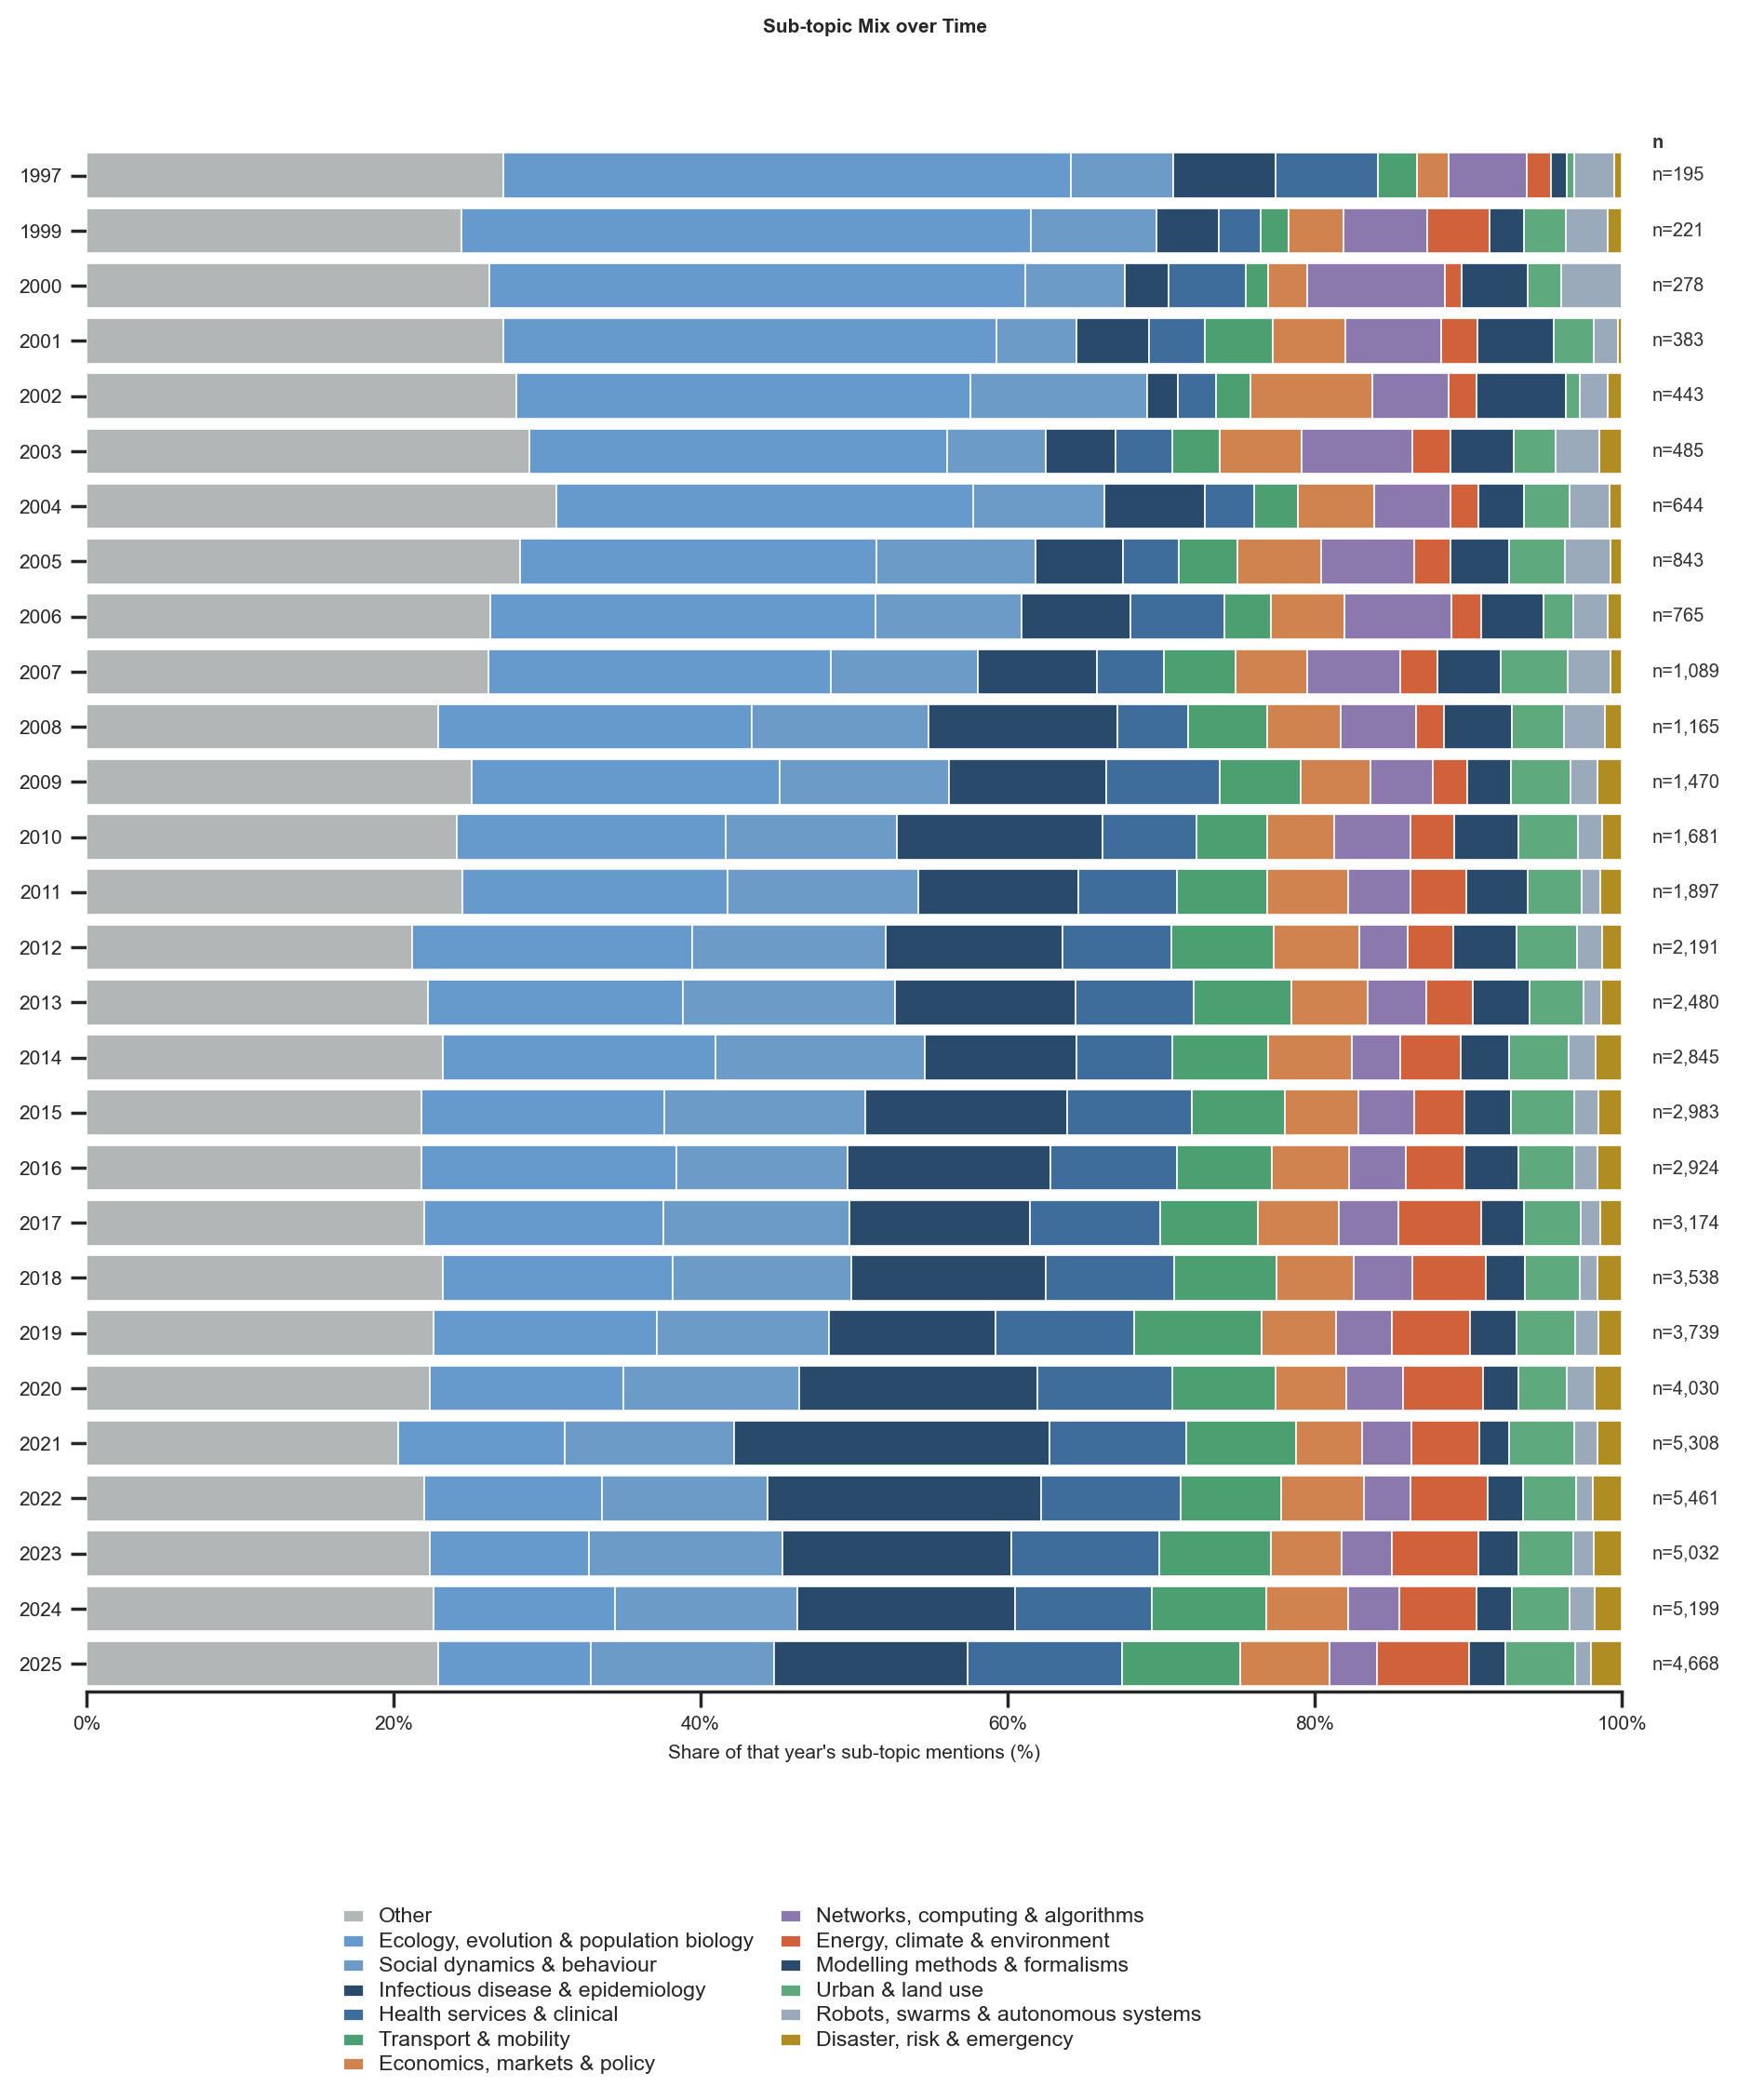
\includegraphics[width=0.96\textwidth,height=0.78\textheight,keepaspectratio]{figures/figure_06.png}
\setcounter{figure}{5}
\caption{Annual evolution of subtheme composition, 1997–2025.}
\label{fig:figure6}
\end{figure}

The annual subtheme series traces this diversification over time. Ecology, evolution, and population biology make up a smaller share of recent annual mentions, while infectious disease and epidemiology and social and behavioural topics account for larger shares. Energy, urban systems, networks, and modeling methods remain smaller but visible parts of the mix. Because the figure reports each year’s share of subtheme mentions, it describes changes in relative emphasis, not absolute publication counts.

Topic co-occurrence offers another view of the corpus’s breadth. Epidemiology/public health co-occurs with health-care systems in 4,476 papers; ecology/environment with policy and disaster response in 2,585; and urban/land-use planning with transport in 1,939 and energy systems in 1,075. These pairings show that many papers are indexed across intersecting application areas rather than isolated topics. Co-occurrence does not, by itself, establish that the topics are integrated within the same model or that one domain influences another.

\begin{figure}[htbp]
\centering
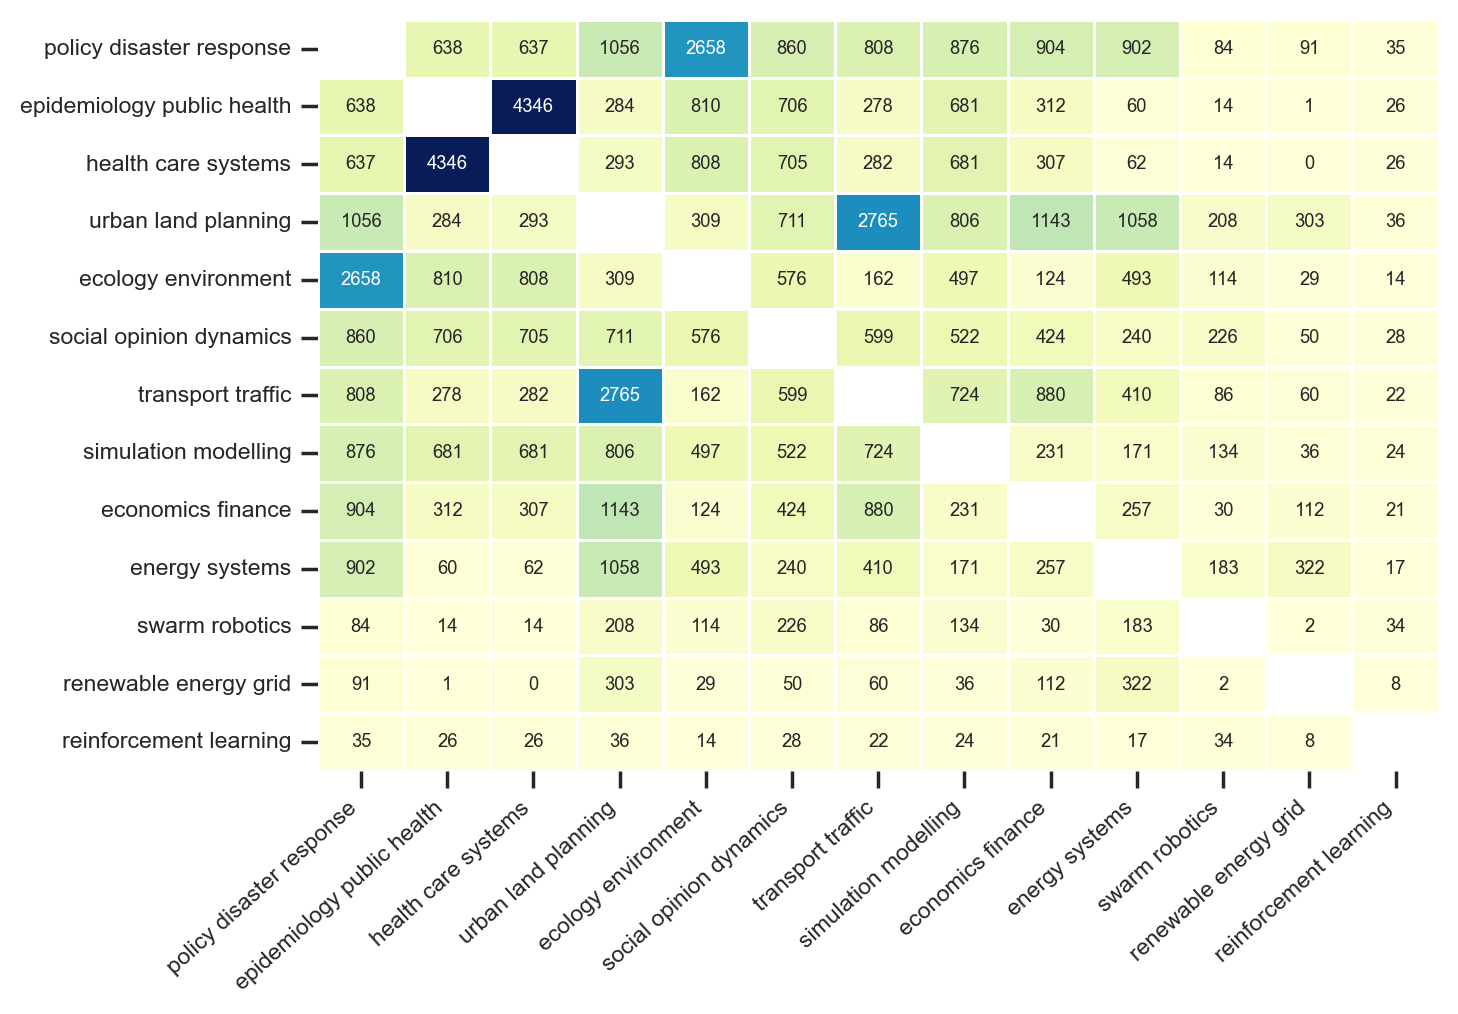
\includegraphics[width=0.96\textwidth,height=0.78\textheight,keepaspectratio]{figures/figure_07.png}
\setcounter{figure}{7}
\caption{Cross-domain co-occurrence intensity.}
\label{fig:figure8}
\end{figure}

This co-occurrence structure reflects ABM’s transferability across disciplinary settings. Its core concepts—heterogeneous agents, local interaction, adaptation, and emergence—can be used to study many kinds of complex systems. The observed links among health, urban systems, transport, environmental processes, and social dynamics therefore suggest that an increasing share of the literature addresses coupled problems. Some models may represent interactions among people, institutions, infrastructure, and the environment, allowing researchers to examine feedback and unintended consequences that aggregate approaches can obscure. The co-occurrence results indicate topical overlap, however, and should not be taken as direct evidence that every paper models these mechanisms jointly.

\subsection{The changing object of simulation}

Humans and households account for 41.20\% of modeled-entity classifications, while patients and other biological entities account for 22.34\%. Decade-based logistic models show a strong increase in human/household representation (OR = 1.483 per decade, q = 1.3 × 10−57) and declines in generalized network nodes, software/computational agents, patients/biological entities, and swarm robots. This shift does not imply that computational or biological models are disappearing. Rather, it signals a growing emphasis on coupled human–environment and human–technology systems, where decisions and interaction networks are themselves part of the causal explanation.

\begin{figure}[htbp]
\centering
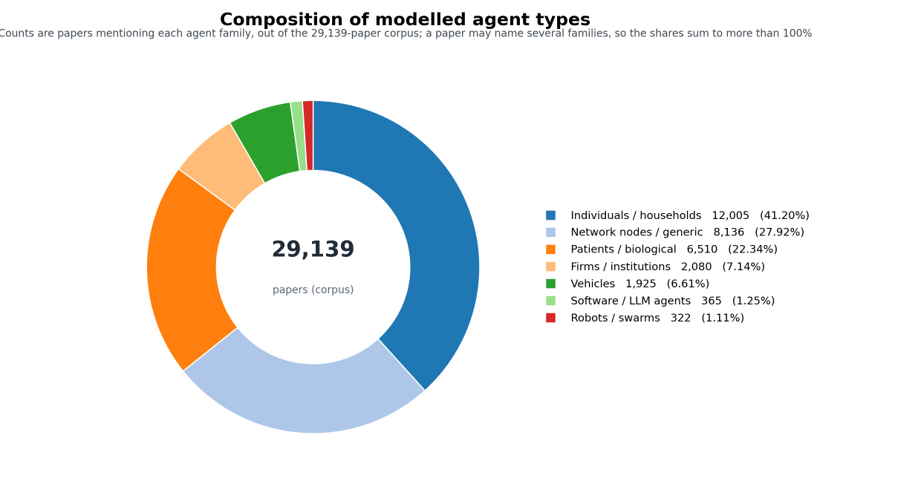
\includegraphics[width=0.96\textwidth,height=0.78\textheight,keepaspectratio]{figures/figure_08.png}
\setcounter{figure}{8}
\caption{Overall composition of modeled agent types.}
\label{fig:figure9}
\end{figure}

\begin{figure}[htbp]
\centering
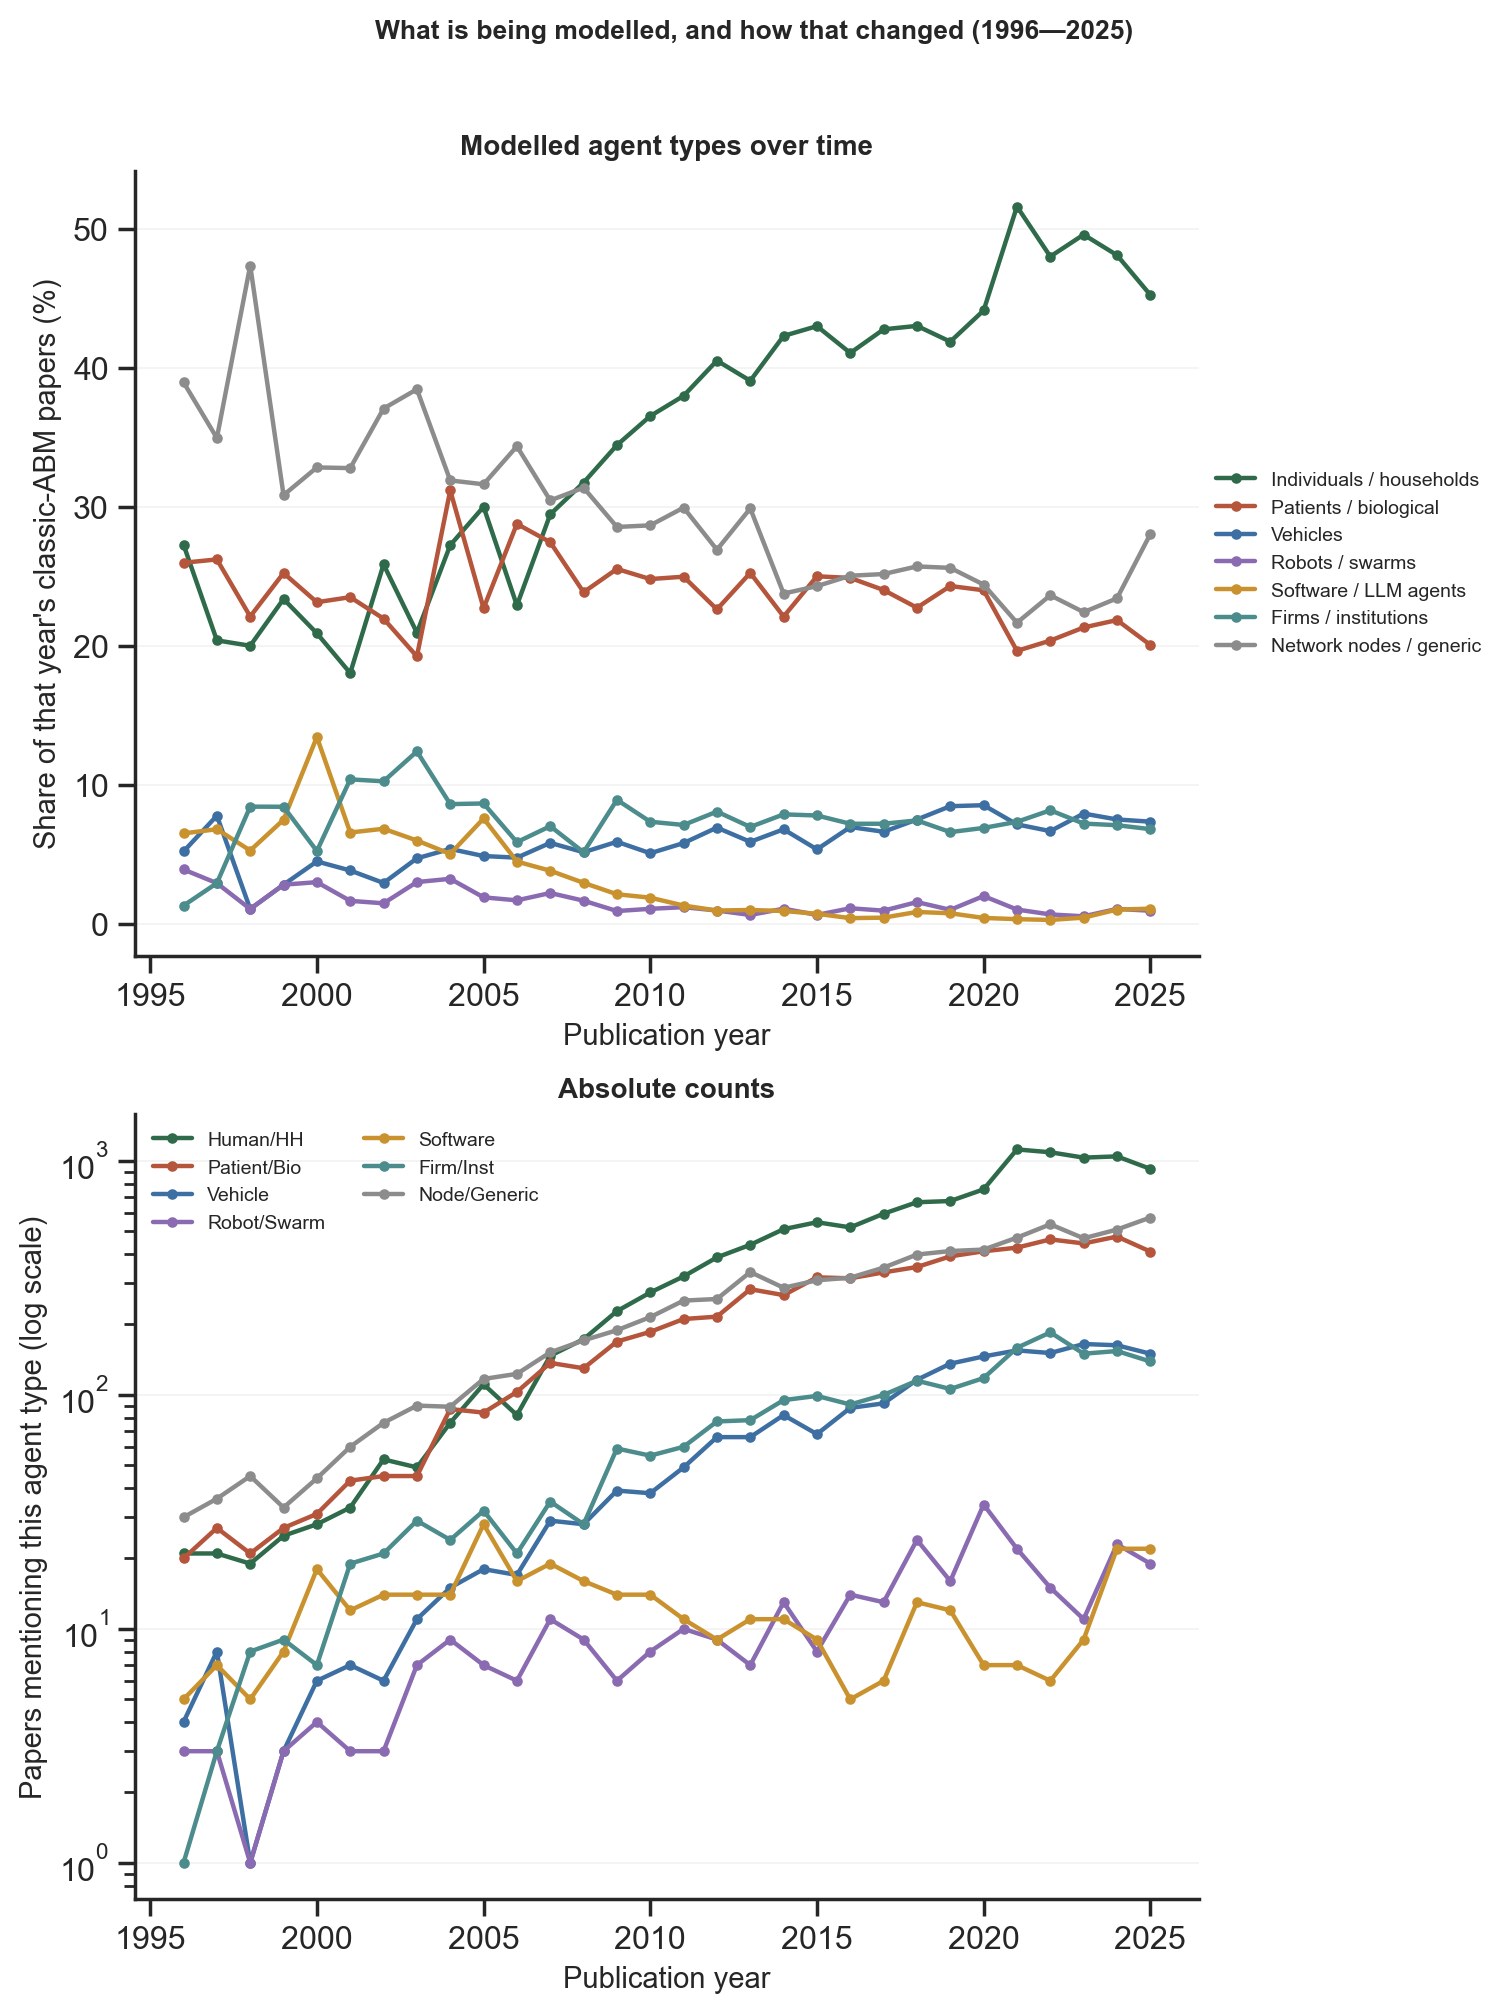
\includegraphics[width=0.96\textwidth,height=0.78\textheight,keepaspectratio]{figures/figure_09.png}
\setcounter{figure}{9}
\caption{Annual trends in modeled agent types, 1996–2025.}
\label{fig:figure10}
\end{figure}

The shift toward human-centered applications sharpens a methodological tension: richer behavioral representations also increase the burden of validation. The ODD protocol and its updates make model structure, design concepts, and implementation details inspectable. As behavioral assumptions become more elaborate, transparent reporting becomes more important, not less. \footnote{Grimm, V., Berger, U., Bastiansen, F., Eliassen, S., Ginot, V., Giske, J., et al. (2006). A standard protocol for describing individual-based and agent-based models. Ecological Modelling, 198(1–2), 115–126. https://doi.org/10.1016/j.ecolmodel.2006.05.023; Grimm, V., Berger, U., DeAngelis, D. L., Polhill, J. G., Giske, J., \& Railsback, S. F. (2010). The ODD protocol: A review and first update. Ecological Modelling, 221(23), 2760–2768. https://doi.org/10.1016/j.ecolmodel.2010.08.019}
\section{Large language model adoption in agent-based modeling}

\subsection{What changed, and what did not}

For this review, 2018–2022 is treated as the pre-LLM comparison period and 2023–2025 as the post-release observation period, with late 2022 as the historical boundary associated with ChatGPT’s public release. This is a periodization device, not a causal design. A before–after comparison can identify temporal reorientation, but it cannot prove that LLMs caused changes in topic choice or collaboration.

The pre/post comparison shows continuity among the highest-ranked subthemes alongside changes elsewhere in the distribution. Epidemiological modeling and opinion dynamics remain first and second in both periods. Social network analysis rises from fourth to third, social influence from fifth to fourth, urban planning from eleventh to sixth, and ABM as a named method from twelfth to eighth; information diffusion also enters the post-release top twenty. In contrast, population dynamics moves from third to fifth, disease-spread modeling from sixth to eighteenth, cost-effectiveness from seventh to twelfth, and wildlife conservation from tenth to twentieth. These are relative rankings among leading subthemes, not measures of absolute publication volume. The pattern is consistent with greater visibility for networked interaction, influence, and information-related questions, but this descriptive comparison cannot attribute the changes to LLMs or to any single historical event.

\begin{figure}[htbp]
\centering
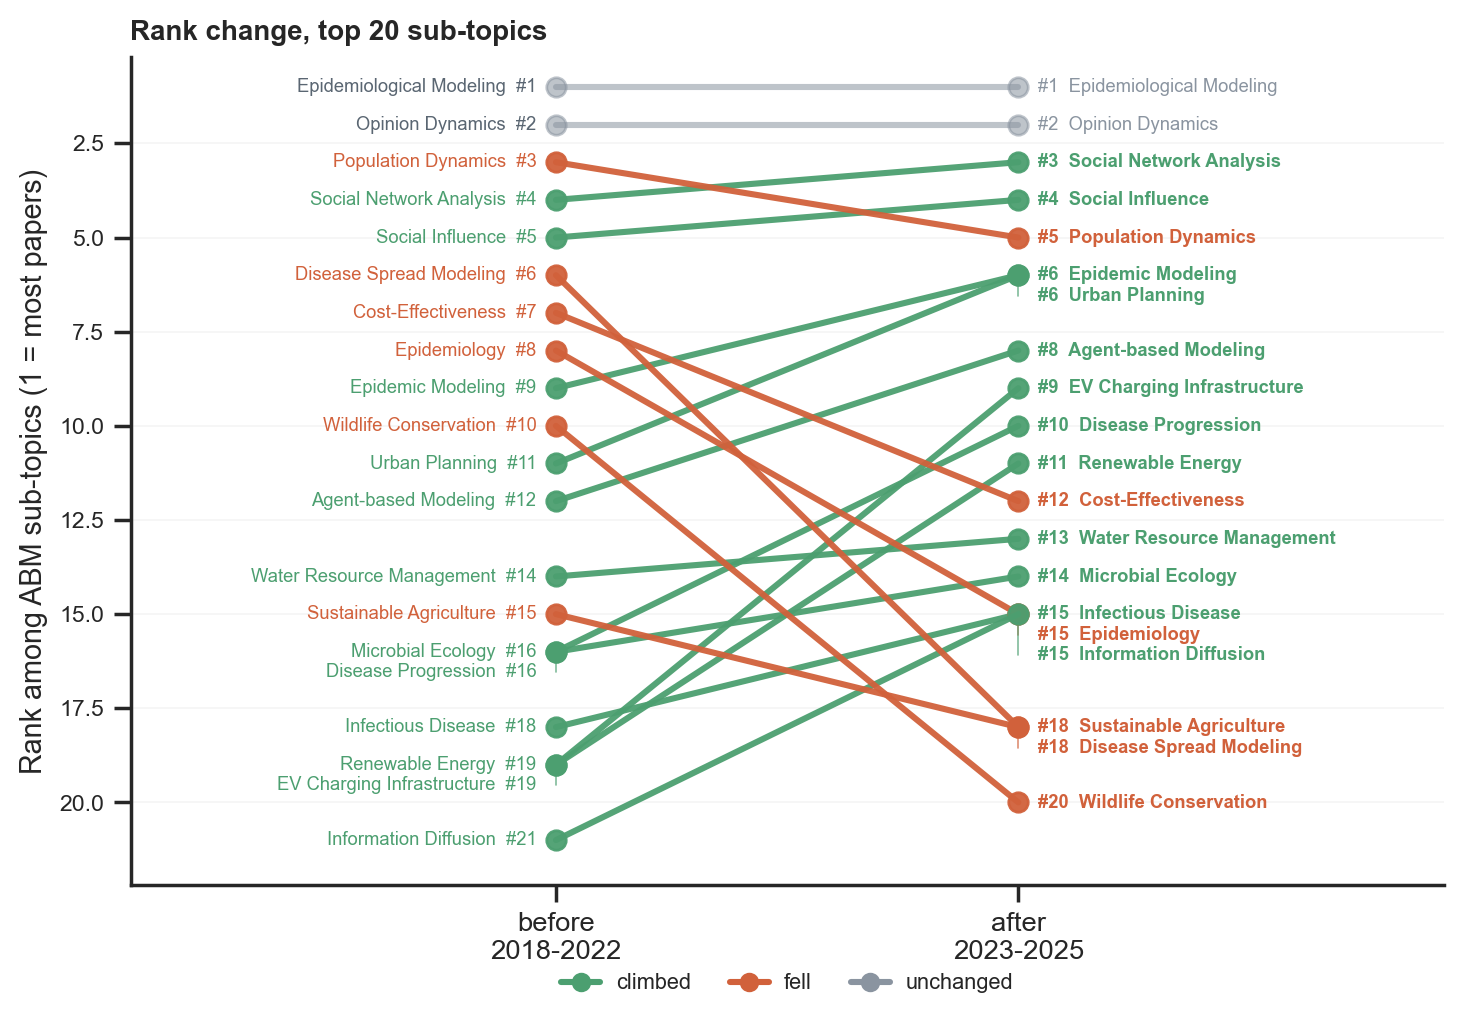
\includegraphics[width=0.96\textwidth,height=0.78\textheight,keepaspectratio]{figures/figure_10.png}
\setcounter{figure}{6}
\caption{Rank changes among leading subthemes before and after the public emergence of ChatGPT.}
\label{fig:figure7}
\end{figure}

\begin{table}[htbp]
\centering
\scriptsize
\setlength{\tabcolsep}{3pt}
\renewcommand{\arraystretch}{1.18}
\setcounter{table}{1}
\caption{}
\label{tab:table2}
\begin{tabularx}{\linewidth}{>{\raggedright\arraybackslash}p{0.15\linewidth} *{4}{>{\raggedright\arraybackslash}X}}
\toprule
\textbf{Dimension} & \textbf{Before LLM diffusion (2018–2022)} & \textbf{Early post-LLM period (2023–2025)} & \textbf{Evidence in corpus} \\
\midrule
Research focus & Population, disease, ecology, and established simulation domains & Social networks, influence, information diffusion, and socio-technical systems & Subtheme rank shifts \\
LLM adoption & Not a regular modeling component & 1.50\% → 2.75\% → 5.65\% annually & Cochran–Armitage trend p < 0.001 \\
Primary role & Hand-coded rules and conventional computational tools & Behavioral rules/decision mechanisms plus tool support & 59.6\% internal; 40.4\% instrumental \\
Modeled entity profile & Humans and biological entities within established ABM traditions & More software/computational agents among LLM papers & Software agents +11.5 pp; biological entities −12.7 pp \\
Collaboration & Growing team science already underway & LLM papers show lower international collaboration & 20.3\% vs 31.6\%; q = 5.5 × 10−4 \\
\bottomrule
\end{tabularx}
\end{table}

Table 2. A descriptive comparison of ABM before and after the public emergence of LLMs. The comparison is associational, not causal.

\subsection{Diffusion is accelerating but remains at an early stage}

LLM use grew rapidly from a small base. Of the 29,139 papers in the corpus through 2025, 236 (0.81\%) were classified as using an LLM. Annual counts increased from 32 in 2023 to 63 in 2024 and 141 in 2025. Using the annual denominator applied in the corpus trend analysis, the corresponding shares rose from 1.50\% to 2.75\% and 5.65\%, a 2025-to-2023 rate ratio of 3.77. Despite this clear increase, LLM use was not standard practice by 2025: most ABM papers in the observation window were not classified as LLM-enabled. Because the post-release series covers only three years, it should be read as an early-diffusion snapshot, not a settled trajectory.

\begin{figure}[htbp]
\centering
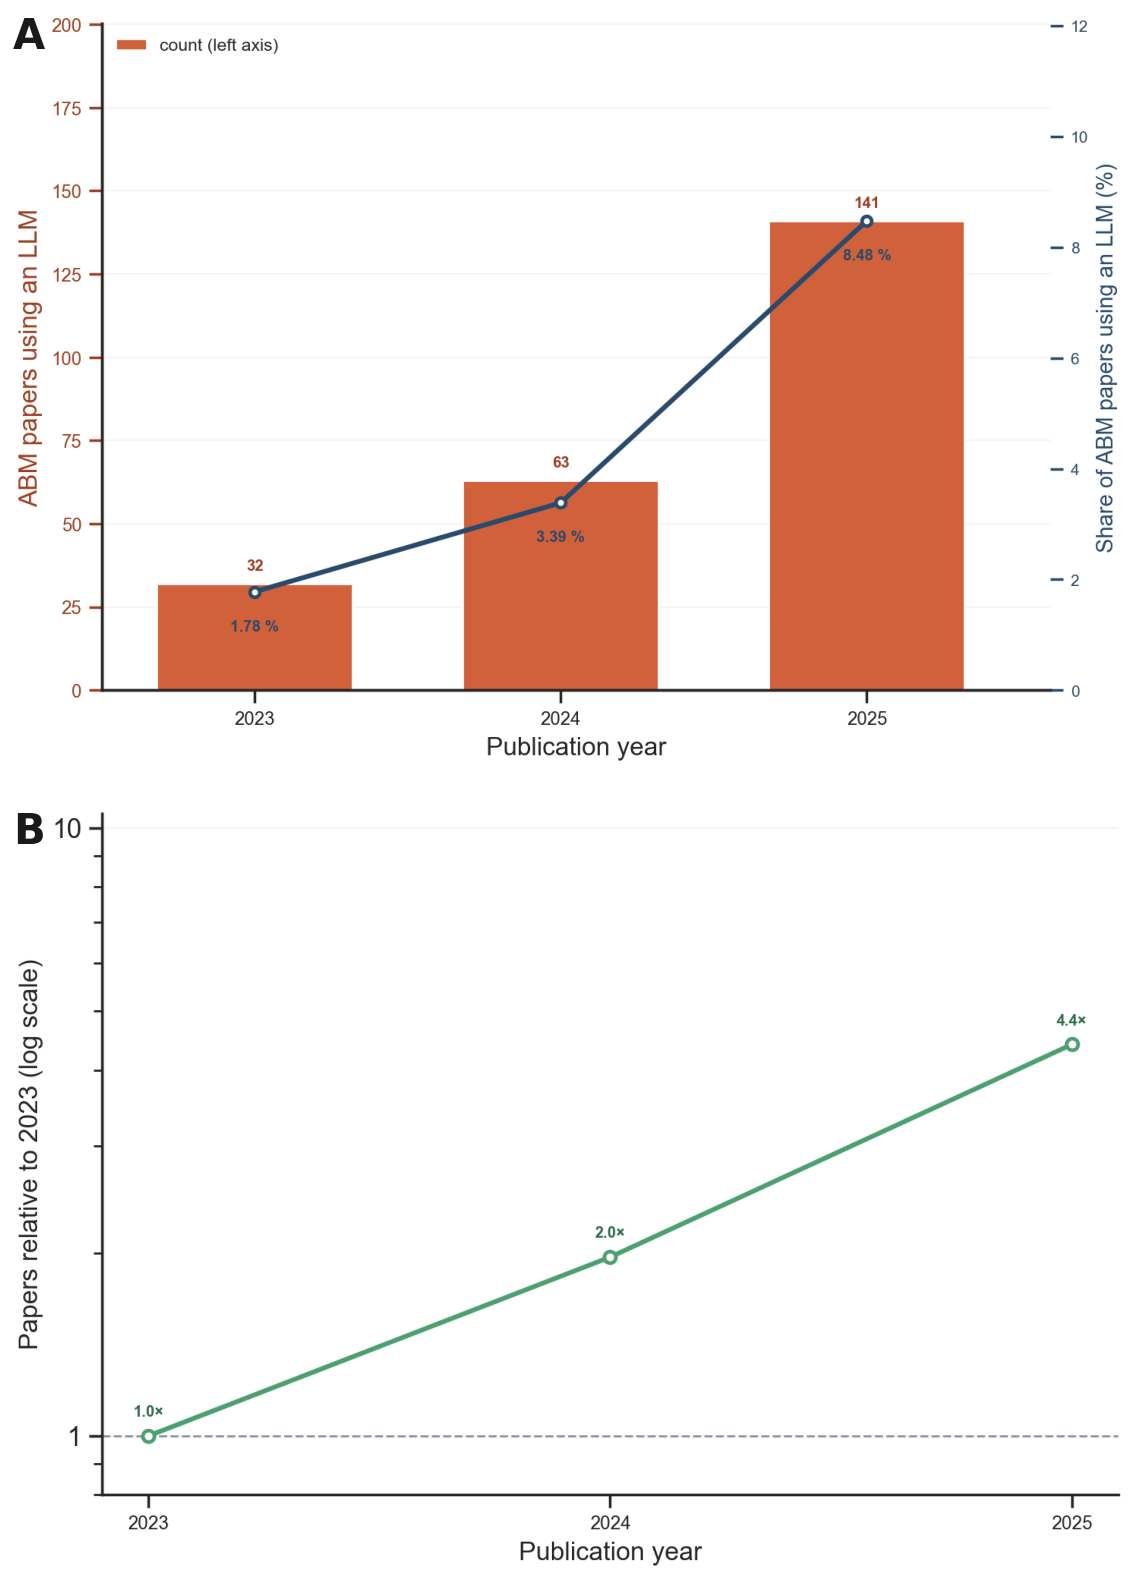
\includegraphics[width=0.96\textwidth,height=0.78\textheight,keepaspectratio]{figures/figure_11.png}
\setcounter{figure}{10}
\caption{LLM adoption over time and index relative to 2023.}
\label{fig:figure11}
\end{figure}

The LLM’s function is as important as its presence. Of 235 papers with a classifiable role, 140 (59.6\%; Wilson 95\% CI 53.2–65.6) used the model in agent behavior or decision-making. The other 95 papers (40.4\%) used LLMs in supporting roles, including code or model implementation, data and parameter generation, evaluation or text analysis, and natural-language interfaces. The corpus thus shows two concurrent patterns: LLMs can form part of the simulated decision mechanism, or support the research workflow around it. These roles should be distinguished because only the former directly changes how simulated agents generate behavior.

\begin{figure}[htbp]
\centering
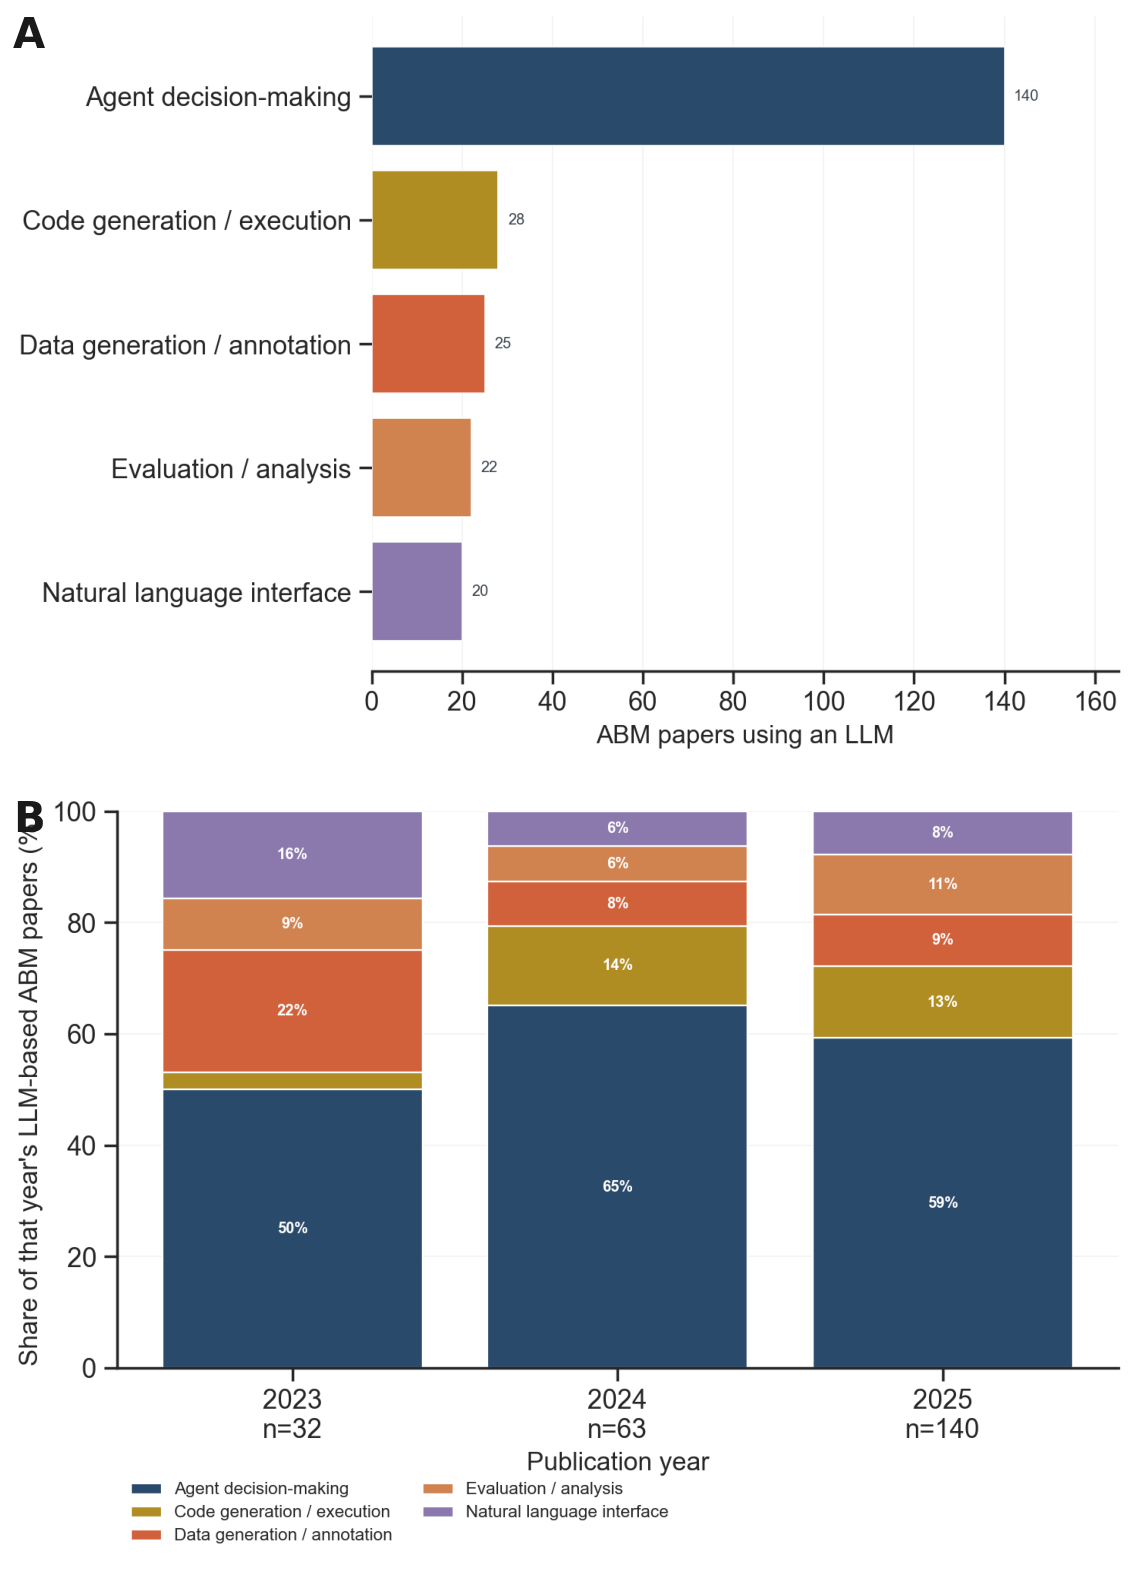
\includegraphics[width=0.96\textwidth,height=0.78\textheight,keepaspectratio]{figures/figure_12.png}
\setcounter{figure}{11}
\caption{Functional roles of LLMs in ABM and their annual composition.}
\label{fig:figure12}
\end{figure}

\begin{figure}[htbp]
\centering
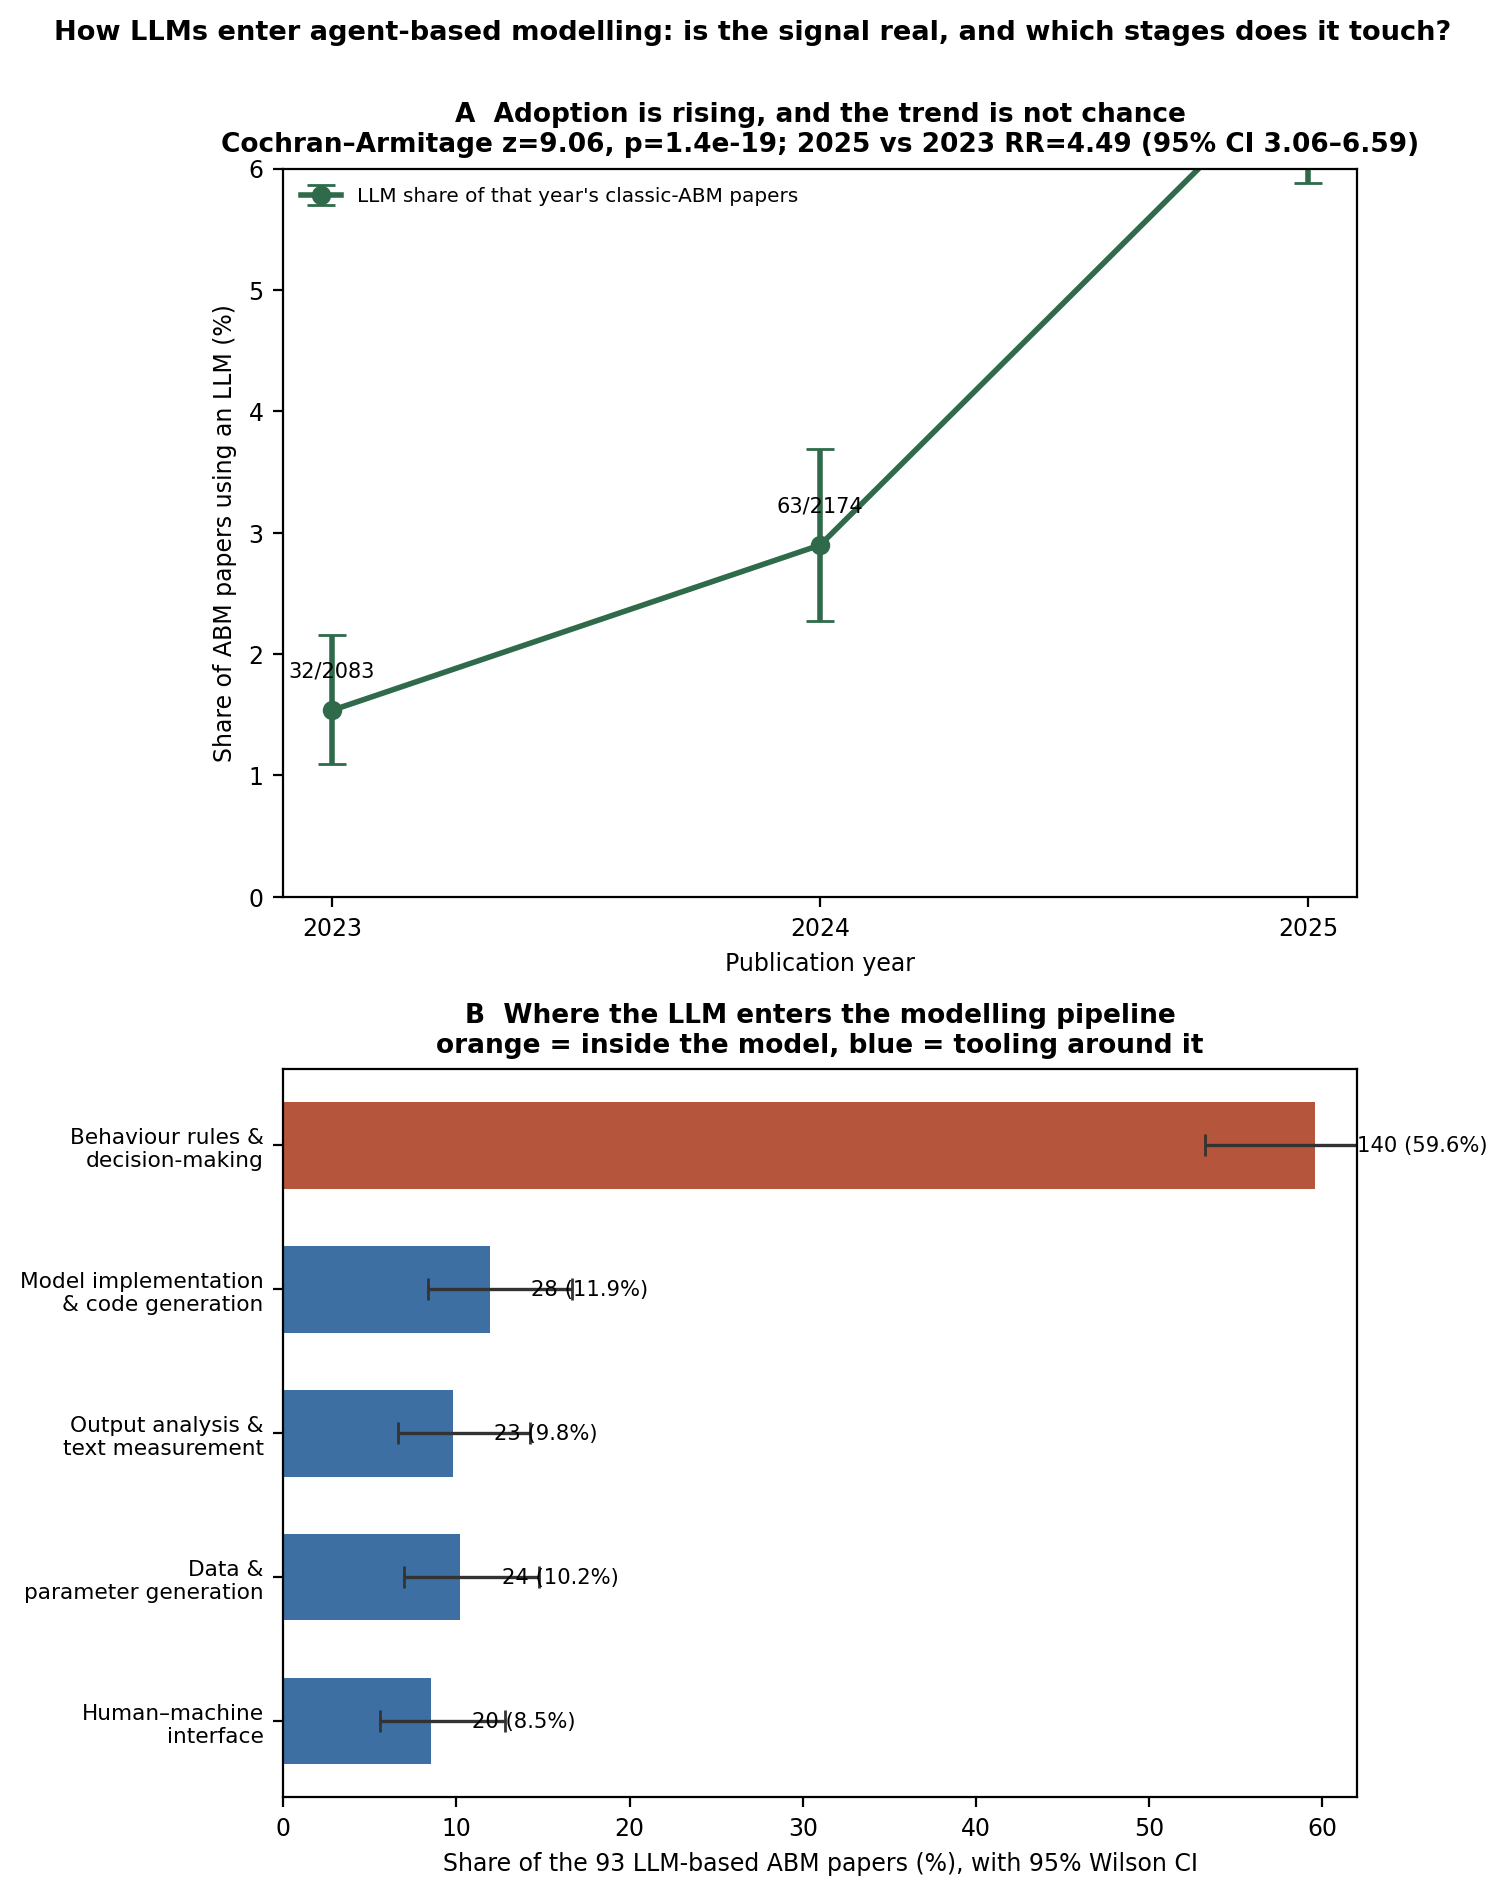
\includegraphics[width=0.96\textwidth,height=0.78\textheight,keepaspectratio]{figures/figure_13.png}
\setcounter{figure}{12}
\caption{Entry points of LLMs into the ABM workflow: adoption tests and modeling-stage location.}
\label{fig:figure13}
\end{figure}

The key transition is the use of LLMs within agents’ decision processes, rather than only as tools for programming, text analysis, or data processing. Conventional ABMs typically specify decision rules directly; LLM-based agents can instead interpret context, retrieve memories, plan, and interact in natural language. Such capabilities may represent flexible, context-dependent behavior that fixed rules are less suited to capture. They do not, on their own, establish that the resulting behavior is valid. \footnote{Park, J. S., O’Brien, J. C., Cai, C. J., Morris, M. R., Liang, P., \& Bernstein, M. S. (2023). Generative agents: Interactive simulacra of human behavior. In Proceedings of the 36th Annual ACM Symposium on User Interface Software and Technology. https://doi.org/10.1145/3586183.3606763} \footnote{Huang, Q., Vora, J., Liang, P., \& Leskovec, J. (2024). Large language models empowered agent-based modeling and simulation: A survey and perspectives. Humanities and Social Sciences Communications, 11, 1259. https://doi.org/10.1057/s41599-024-03611-3; Wang, L., Ma, C., Feng, X., Zhang, Z., Yang, H., Zhang, J., Chen, Z., Tang, J., Chen, X., Lin, Y., Zhao, W. X., Wei, Z., \& Wen, J.-R. (2024). A survey on large language model based autonomous agents. Frontiers of Computer Science, 18(6), 186345. https://doi.org/10.1007/s11704-024-40231-1}

\subsection{Limits of current LLM-enabled ABM and research priorities}

The available evidence supports treating LLM-enabled ABM as an emerging extension of established ABM, not as its replacement. LLM-driven agents still need to represent bounded rationality, adaptation, spatial and network constraints, and institutional rules, and their behavior must be calibrated and validated against empirical evidence. Linguistically coherent, contextually plausible responses are not necessarily stable or behaviorally valid: agents may produce inconsistent choice probabilities, weak demographic differentiation, or implausible policy responses. Outcomes may also vary with model version, prompt, context, stochastic settings, and knowledge-updating procedures. These issues are especially consequential when an LLM serves as the decision engine, because even small changes can alter the simulated behavioral mechanism. \footnote{Ghaffarzadegan, N., Majumdar, A., Williams, R., \& Hosseinichimeh, N. (2024). Generative agent-based modeling: An introduction and tutorial. System Dynamics Review, 40(1), e1761. https://doi.org/10.1002/sdr.1761; Lu, Y., Aleta, A., Du, C., Shi, L., \& Moreno, Y. (2024). LLMs and generative agent-based models for complex systems research. Physics of Life Reviews, 51, 283–293. https://doi.org/10.1016/j.plrev.2024.10.013}

Future research should make uncertainty and validity assessable. Studies should compare LLM-based agents with rule-based and empirically calibrated baselines, then test sensitivity to model version, prompt, random seed, temperature, and information-retrieval strategy. Validation should draw on observed behavior, experiments, or historical cases and should assess both individual decisions and aggregate outcomes. Researchers should also report computational costs, data provenance, privacy safeguards, and how generated outputs were reviewed. Current applications are concentrated in a limited set of areas and cover only the first years of adoption; cross-domain replications and longer time series are therefore needed before general claims about LLMs’ value in ABM are justified.

\emph{Figure 14. Cross-distribution of application domains and LLM roles.}

\subsection{Application domains and simulated agent types}

LLM-enabled ABM is concentrated in a few application areas. Among the 235 papers with classifiable roles in Figure 14, social and opinion dynamics is the largest group (81 papers; 34.5\%), followed by health and epidemiology (58; 24.7\%). Other prominent areas are AI and multi-agent computing (28; 11.9\%), policy and disaster response (25; 10.6\%), sustainability and energy (21; 8.9\%), and transport and urban mobility (18; 7.7\%). Networks and communication and other specialized domains contribute two papers each. This distribution places current work chiefly in social-behavioral and health research, alongside a smaller technical strand in AI and multi-agent systems. Decision-making is the most common LLM function across the major domains; coding, data generation, analysis, and interfaces provide additional routes of use.

The agent types represented in LLM-related studies also differ from those in the broader ABM corpus. Software or computational agents are 11.5 percentage points more prevalent, while biological entities are 12.7 points less prevalent, in the LLM subset. This is consistent with the emergence of software and LLM-based agents as objects of study, but it does not mean that every paper using an LLM simulates an LLM agent. Some use the model to support decisions, data preparation, analysis, or interaction for a different agent population. Separating the LLM’s function from the simulated agent type is therefore essential to interpreting the field’s development.

\subsection{An evaluative framework for LLM-enabled ABM}

The review proposes evaluating LLM-enabled ABM along four dimensions. Behavioral validity asks whether an LLM agent reproduces observed choices, response times, network ties, and switching behavior. Process validity examines whether mechanisms such as memory, planning, social influence, and adaptation remain stable under changes to prompts, seeds, models, or temperature. Macro-level validity tests whether aggregate patterns and policy responses match historical or experimental benchmarks. Governance validity concerns provenance, disclosure of synthetic decisions, protection of sensitive data, and replicability. This framework complements ODD-style documentation with model cards, prompt and version records, stochastic controls, and behavioral benchmarks.
\section{Collaboration networks: formation, bridges, and disciplinary exchange}
\label{sec:collaboration}

\subsection{Corpus and network construction}

The collaboration analysis was rebuilt from the same 29,139-record, 1972--2025 corpus used for the review's publication and topic results. Two records have no usable publication year. Among the dated records, two duplicate document identifiers were collapsed, leaving 29,135 unique dated records. Author lists were available for 29,016 of these. The remaining 119 records were retained in the review corpus but could not contribute author--author links. These counts distinguish the corpus denominator from the observable coauthorship denominator.

Author names were canonicalized with the same identity rules used in the earlier analysis, while preserving byline order for BAL author-position credit. An undirected edge joins two authors who appear on the same paper. Following the original network algorithm, a paper with $n$ authors adds $1/(n-1)$ to each of its coauthor edges; repeated joint papers accumulate weight. This reduces the influence of a single large team while preserving repeated collaboration. Core authors were selected by the original BAL measure, the mean rank of position-weighted fractional output and domain/year-normalized summed citations. The top 800 BAL authors were retained, isolated authors were removed, and the largest connected component was used for the community map. Weighted Louvain detection used the original deterministic partition routine and resolution 1.0. The temporal analysis uses the full observable author network, rather than only this selected core.

The complete coauthorship graph contains 70,603 authors with at least one coauthor and 271,869 distinct pairs. Its largest connected component contains 42,425 authors, or 60.1\% of coauthor nodes. Among the BAL top 800, 630 remain after isolates are removed; their largest component has 554 authors and 1,446 links. Weighted Louvain yields 36 communities with modularity $Q=0.8924$. These values replace the previous estimates obtained from the smaller 23,280-paper network. Figure~\ref{fig:collab_communities} shows the rebuilt core with every author named. A companion SVG vector figure supports zooming to read individual names.

\begin{figure}[htbp]
\centering
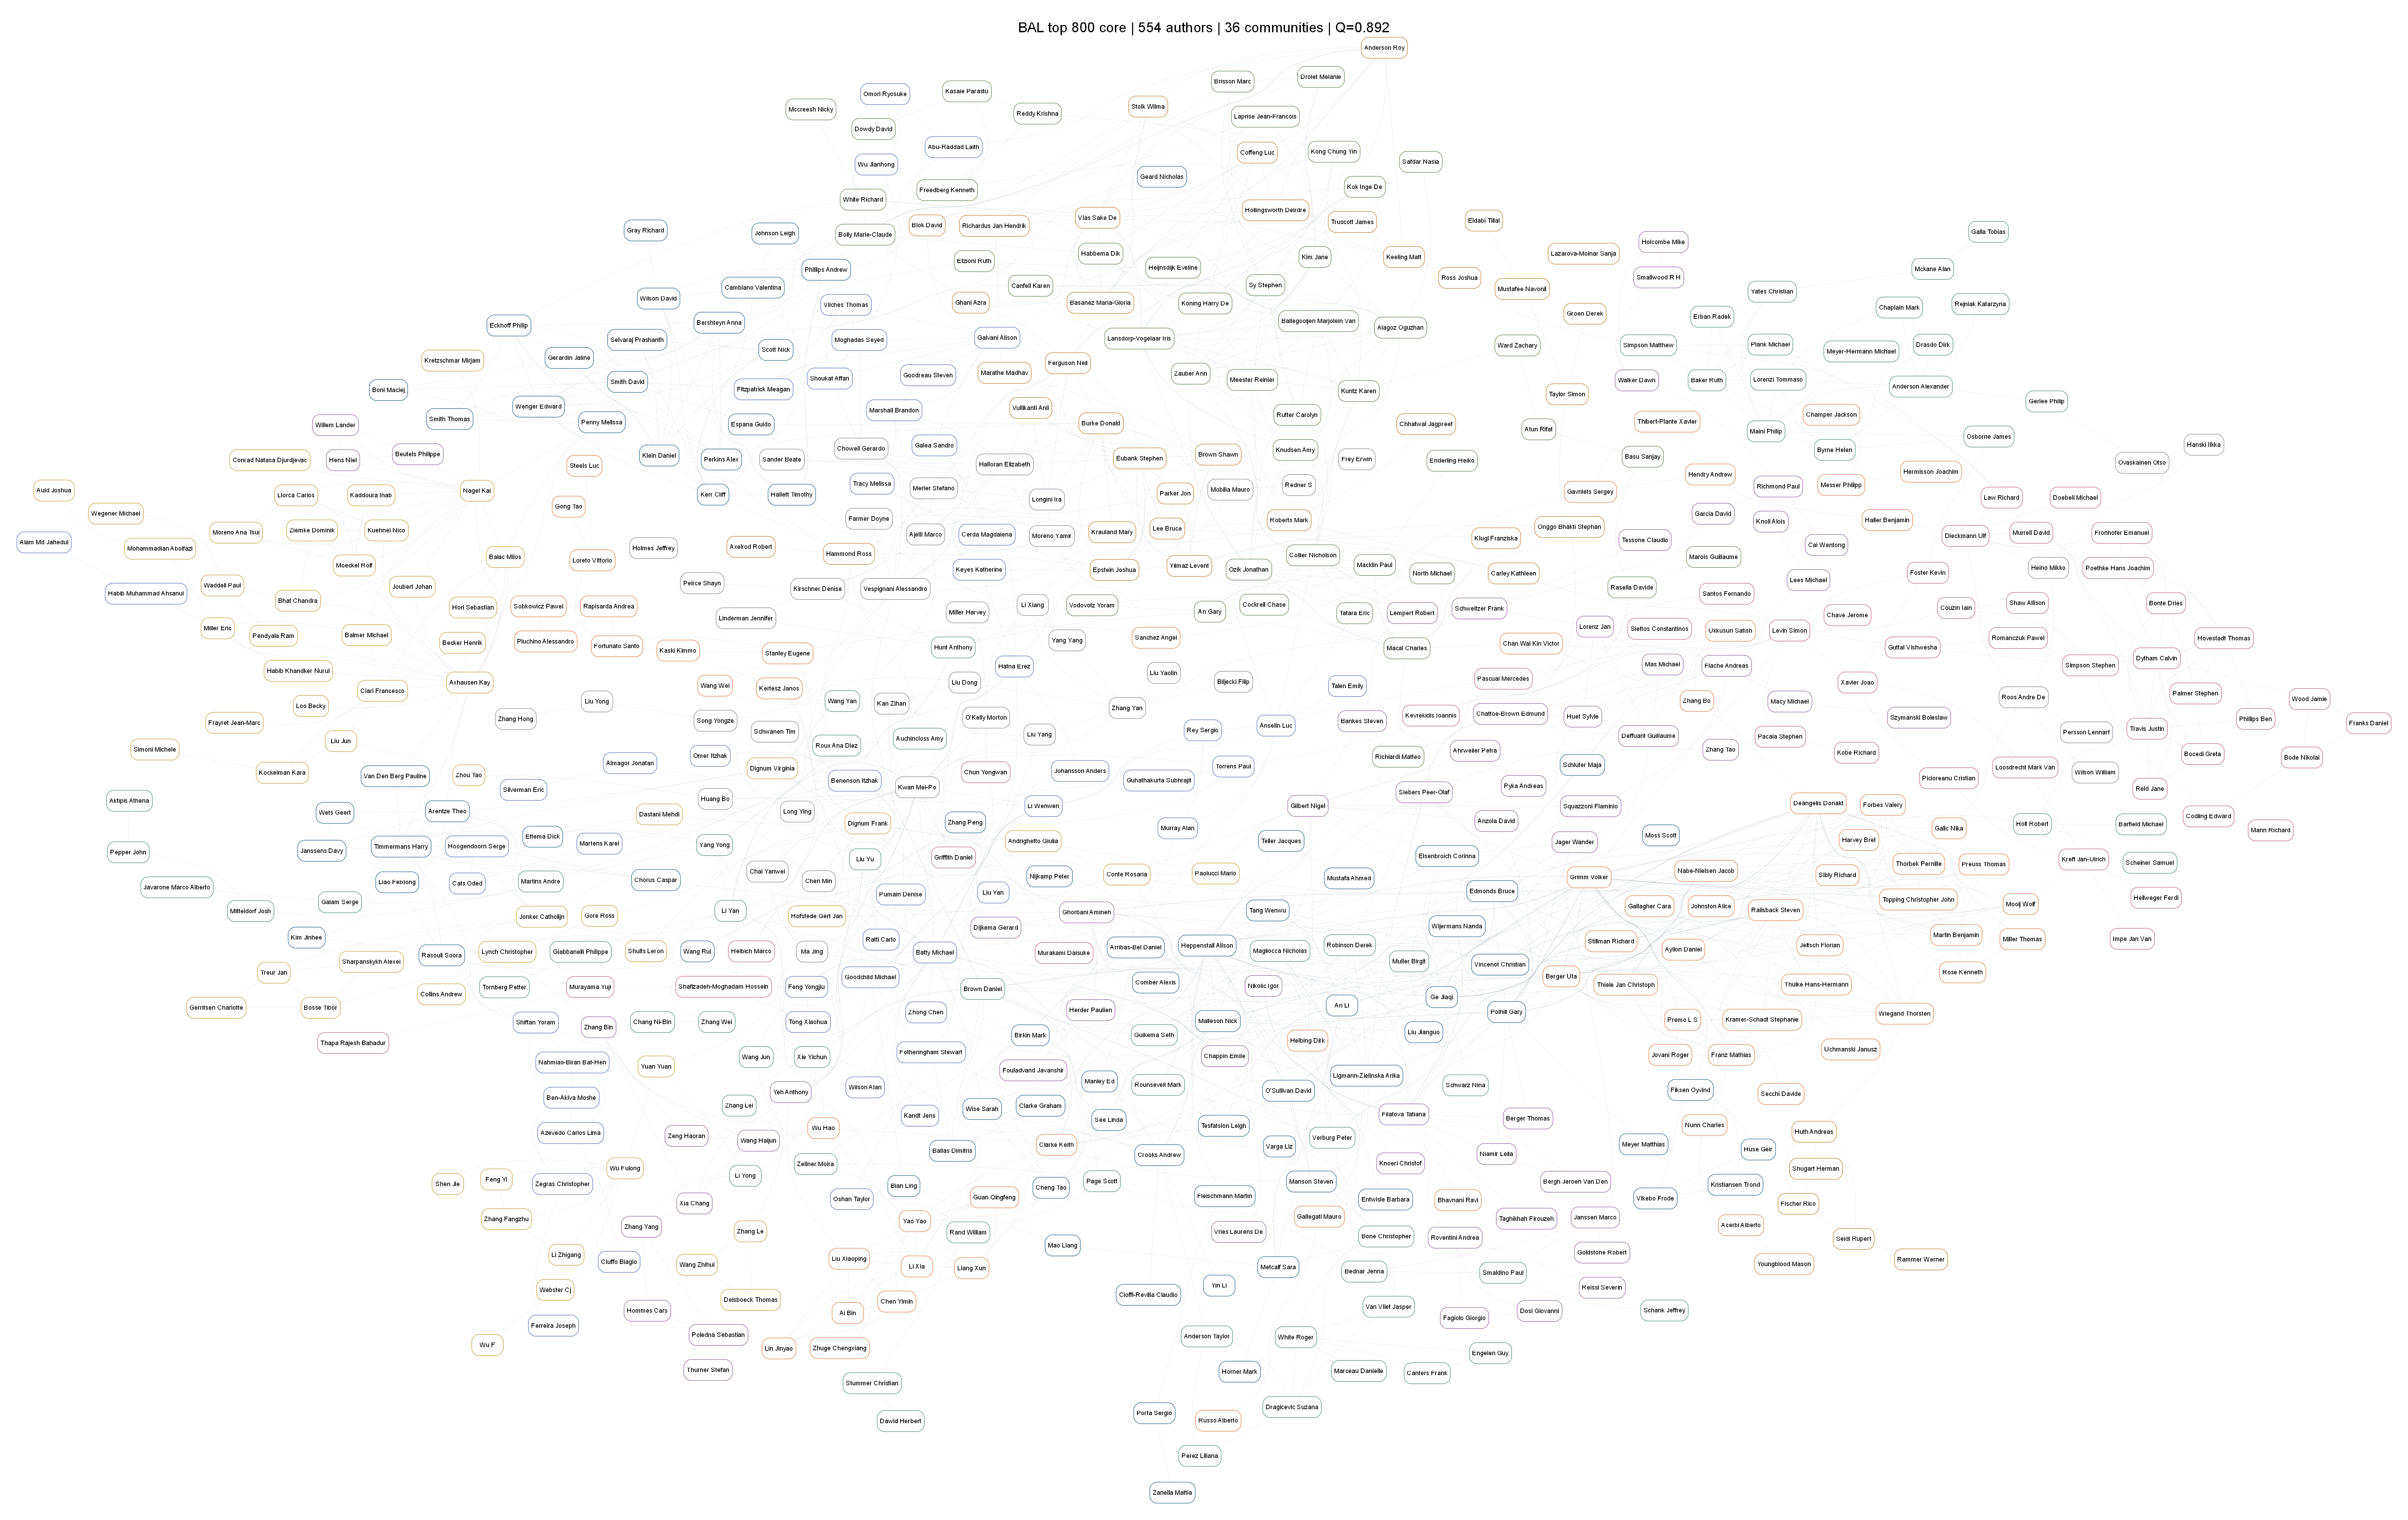
\includegraphics[width=0.94\textwidth,height=0.75\textheight,keepaspectratio]{figures/collab_29139_author_communities.png}
\setcounter{figure}{13}
\caption{Fully labelled author collaboration core from the 29,139-record corpus. Every one of the 554 authors in the largest connected component of the BAL top 800 is named. Box outline color indicates weighted Louvain community, and lines indicate coauthorship. The separate SVG version is intended for close reading at full resolution.}
\label{fig:collab_communities}
\end{figure}

\subsection{Formation and persistence of collaboration}

To distinguish expansion from continuity, we counted a distinct author pair once within each time period. A \emph{new pair} had not appeared in any earlier period; a \emph{repeated pair} had appeared previously. Consecutive-period survival is the fraction of pairs in the preceding period that reappear in the next. The periods retain the earlier manuscript's breakpoints. Because the intervals have unequal lengths, new-pair counts are also shown per year and survival rates should be read as descriptive period summaries rather than standardized hazards.

\begin{table}[htbp]
\centering
\small
\setlength{\tabcolsep}{5pt}
\caption{Formation and persistence of coauthorship ties in the observable network}
\label{tab:collab_temporal}
\begin{tabular}{lrrrrrr}
\toprule
Period & Papers & Authors & New pairs & Repeated pairs & Prior ties surviving & Largest component \\
 & & & per year & (\% of current) & (\%) & (\% of authors) \\
\midrule
1972--2005 & 1,862 & 3,594 & 181 & 0.0 & --- & 5.2 \\
2006--2012 & 4,577 & 10,377 & 3,276 & 1.2 & 4.5 & 12.3 \\
2013--2015 & 3,603 & 9,941 & 7,577 & 6.0 & 6.1 & 10.9 \\
2016--2025 & 18,974 & 54,576 & 22,006 & 1.6 & 12.1 & 54.7 \\
\bottomrule
\end{tabular}
\end{table}

\begin{figure}[htbp]
\centering
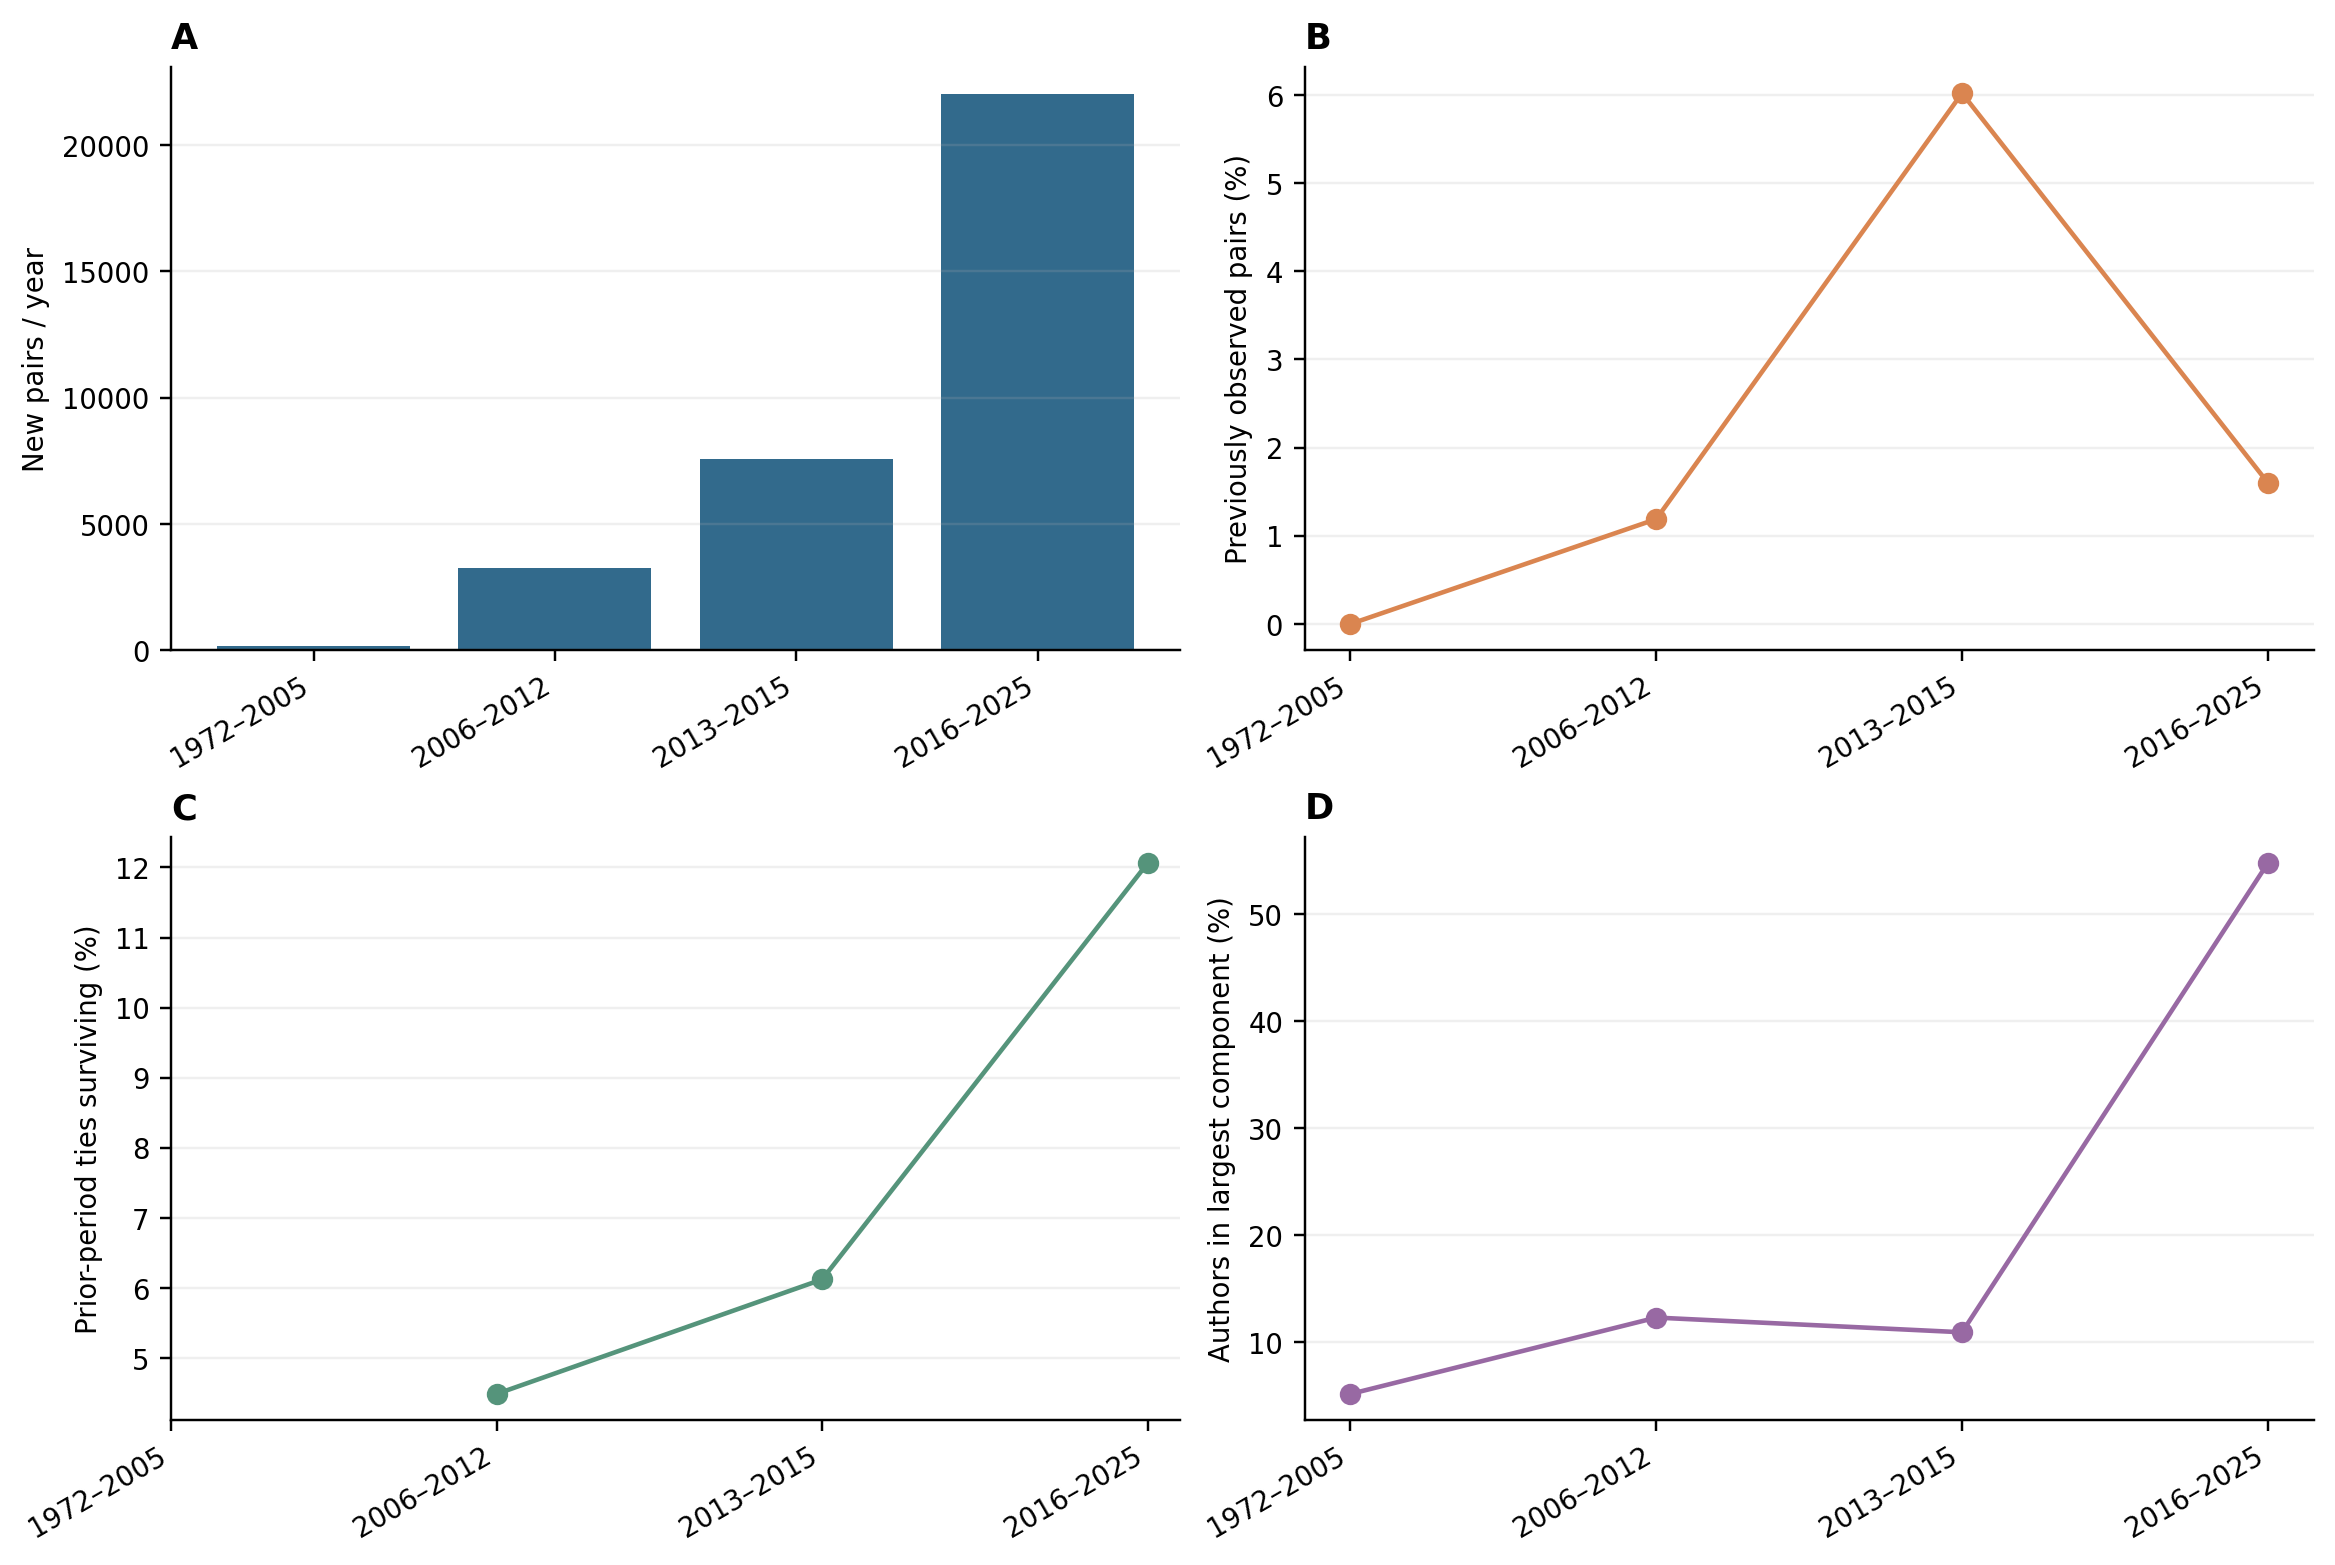
\includegraphics[width=0.96\textwidth,height=0.78\textheight,keepaspectratio]{figures/collab_29139_temporal_ties.png}
\caption{New and repeated coauthor pairs, adjacent-period tie survival, and the largest-component share. The periods follow the previous analysis and have different durations.}
\label{fig:collab_temporal}
\end{figure}

New collaborations accelerated sharply: 6,149 distinct pairs first appeared by 2005, compared with 22,934 in 2006--2012, 22,731 in 2013--2015, and 220,055 in 2016--2025. The annualized figures in Table~\ref{tab:collab_temporal} account for the different period lengths. Yet most links in every later interval were newly observed. Only 1.6\% of pairs active in 2016--2025 had been seen in an earlier period. This low repeated-pair share partly reflects the influx of new authors and should not be interpreted as evidence that established teams ceased collaborating. Of pairs present in 2013--2015, 12.1\% recur in 2016--2025, higher than the preceding adjacent-period overlap. The later interval is longer, which also increases the opportunity to observe a recurrence.

The largest-component share rose from 5.2\% in the first period to 54.7\% in 2016--2025. This indicates that more authors became connected through chains of coauthorship, even though the directly repeated ties remained a small fraction of the rapidly growing edge set. The temporary decrease from 12.3\% in 2006--2012 to 10.9\% in 2013--2015 cautions against describing the trajectory as uniformly monotonic. Figure~\ref{fig:collab_temporal} separates these four aspects of growth.

\subsection{Community boundaries and bridge authors}

High modularity describes a field organized around comparatively dense local collaboration. It does not mean the groups are completely isolated. In the 554-author core, 355 of 1,446 links (24.6\%) cross a Louvain community boundary, but these links carry only 6.2\% of total collaboration weight. Cross-community contacts therefore tend to involve fewer repeated joint papers than within-community contacts. An unweighted Louvain run on the same core still finds 36 communities, with $Q=0.6971$; the difference in modularity shows that repeated collaboration strengthens the observed boundaries.

Two measures identify different roles in connecting this structure. Betweenness centrality counts how often an author lies on shortest paths between other authors. The participation coefficient, $P_i=1-\sum_c(s_{ic}/s_i)^2$, measures how evenly the author's weighted ties are distributed across communities. Michael Batty has high betweenness (0.119) and participation (0.566), consistent with a bridge role in this selected graph. Bruce Edmonds (0.053; 0.663), Peer-Olaf Siebers (0.057; 0.632), Virginia Dignum (0.069; 0.588), and Amineh Ghorbani (0.103; 0.462) also combine path brokerage with diverse community ties. In contrast, Volker Grimm has even higher betweenness (0.207) but lower participation (0.294), and Kay Axhausen has participation of 0.121. Their importance to paths through the graph is therefore distinct from how broadly their direct collaboration is distributed across communities. These are positions within the BAL-selected coauthorship graph, not measures of individual scientific merit.

\begin{figure}[htbp]
\centering
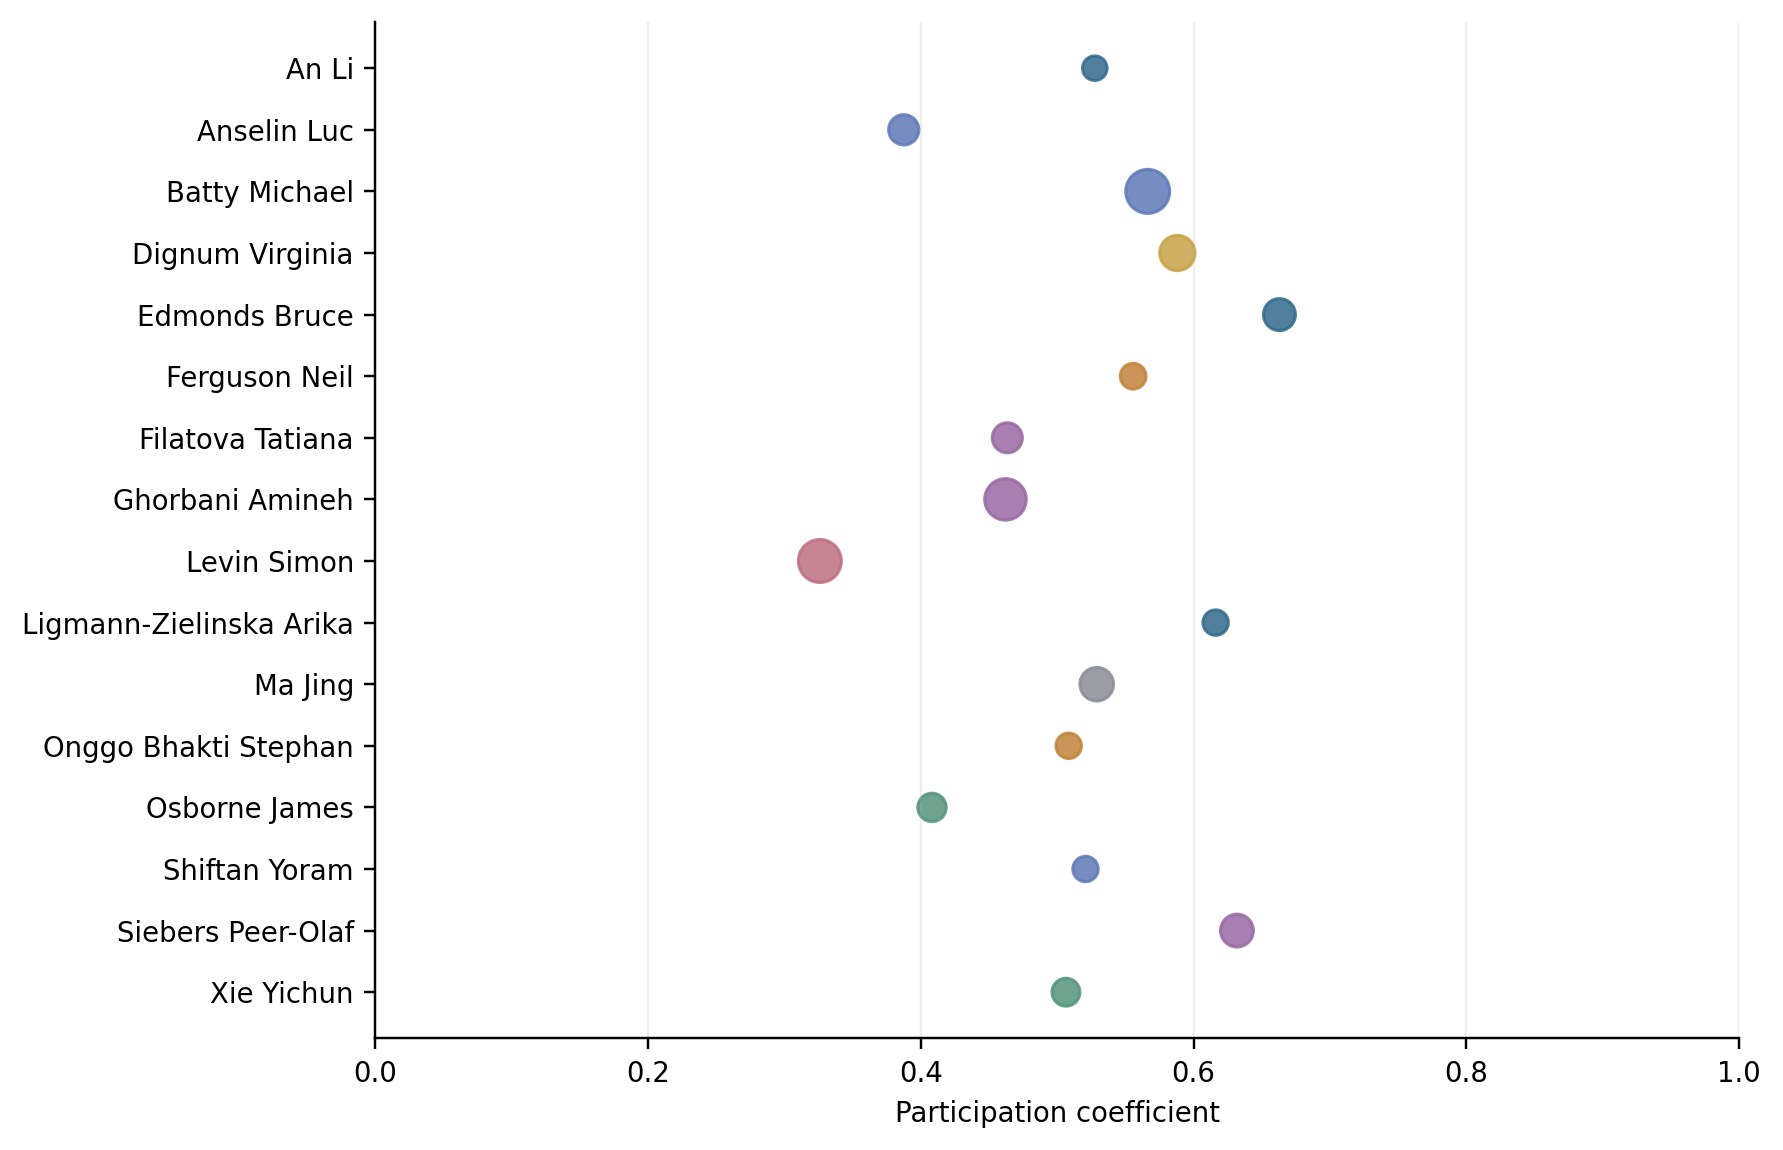
\includegraphics[width=0.90\textwidth,height=0.75\textheight,keepaspectratio]{figures/collab_29139_bridge_authors.png}
\caption{Authors combining high path betweenness and participation across communities. Bubble area reflects betweenness; horizontal position gives the participation coefficient.}
\label{fig:collab_bridges}
\end{figure}

\subsection{Cross-domain collaboration}

We linked each detected community to the primary topics of papers authored by its members. Some communities have clear concentrations: environmental research accounts for 75.8\% of papers associated with community C2, public health for 89.3\% of C8, and transport for 66.1\% of C5. Others are heterogeneous. The leading topic in C1 accounts for only 22.3\%, and that in C3 for 28.6\%; these groups should not be assigned a single disciplinary identity. For descriptive community-to-community comparisons, we labelled a group by its modal topic only when that topic covered at least 35\% of its associated papers.

To test whether collaboration itself spans fields, we also assigned each author a primary domain from the plurality of their papers in the observable corpus. Among multi-author papers for which at least two authors could be assigned domains, the share combining authors from different home domains was 18.5\% in 1972--2005, 25.9\% in 2006--2012, 28.4\% in 2013--2015, and 27.4\% in 2016--2025. Thus cross-domain teamwork became more common than in the early period, but the last two periods do not support a continued increase. The author-domain assignment uses the full observation window, so these percentages describe the final corpus retrospectively rather than measuring a time-varying disciplinary identity.

Public health--environment is the largest cross-domain pair in absolute paper-equivalent volume (1,508), followed by public health--social dynamics (634) and public health--transport (534). Transport--urban/land use contributes 363. Energy--urban/land use (16) and energy--swarm/robotics (14) have much smaller observed volumes. These are counts, not opportunity-adjusted collaboration propensities: small fields can have low pair volumes even if their members are relatively willing to collaborate. Figure~\ref{fig:collab_domains} displays both the time trend and the domain-pair matrix.

\begin{figure}[htbp]
\centering
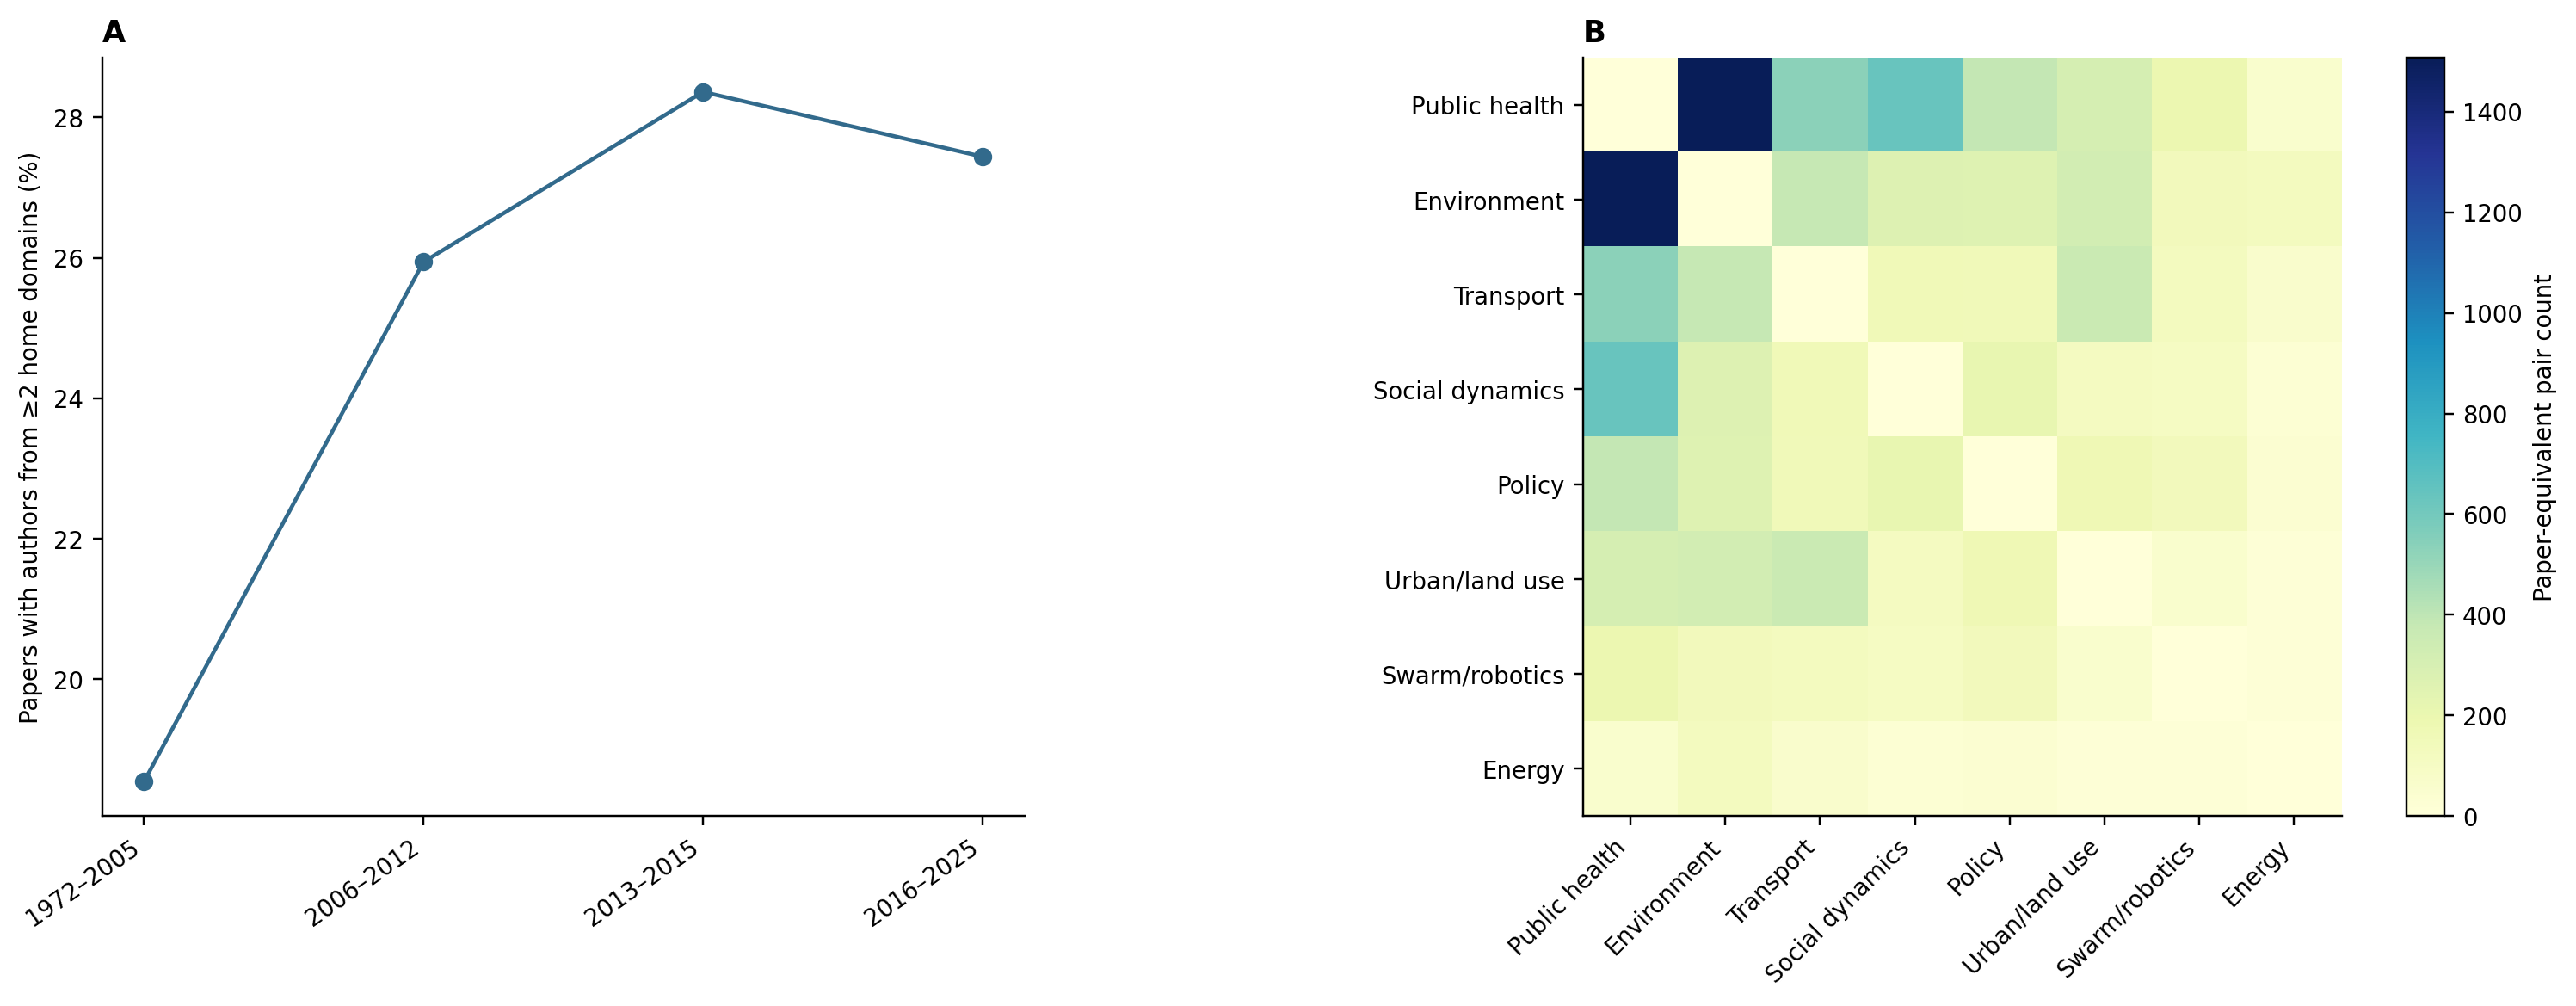
\includegraphics[width=0.98\textwidth,height=0.70\textheight,keepaspectratio]{figures/collab_29139_cross_domain.png}
\caption{Cross-domain coauthorship in the 29,139-record corpus. Panel A shows the share of eligible papers whose coauthors have at least two different primary domains. Panel B shows paper-equivalent coauthor-pair volume across domains; each cross-domain paper contributes total weight one across its different-domain author pairs.}
\label{fig:collab_domains}
\end{figure}

\subsection{Interpretation and limitations}

The expanded corpus portrays a connected but internally structured research field. Large-scale growth has made a majority of coauthor nodes reachable through the largest component, while recurrent collaboration remains concentrated within communities. A subset of authors connects these groups, and the most visible cross-domain paths involve public health, environment, and transport. The distinction between edge presence, repeated edge weight, shortest-path position, and topical mixing is essential: each captures a different form of integration.

The analysis inherits several limits of bibliographic coauthorship data. Canonical name strings can merge distinct people or split one person, author-order credit conventions do not apply equally across fields, and missing author metadata removes 119 unique dated records from network construction. BAL selection is designed to make a readable core and does not represent all 70,603 coauthor nodes. Community labels and modularity depend on this selection and on edge weighting. Finally, a coauthored paper documents a collaboration but does not reveal the direction of knowledge transfer or the quality of intellectual exchange. The figures should therefore be read as a reproducible map of observed collaboration, not as a complete account of disciplinary integration.

\section{Discussion}

\subsection{LLMs as a tool for literature synthesis: scale, semantic reach, and verification}

The corpus-building process illustrates both the value and the limits of LLM-assisted review. Language models can help screen and organize evidence across more publications than reviewers could process manually at the same speed. Used alongside database searches and explicit eligibility criteria, they can support consistent classification of topics, modeled entities, and methodological roles in titles and abstracts. Their semantic capabilities may also distinguish related themes that exact keyword searches or fixed dictionaries overlook, improving thematic discrimination beyond surface-level matching.

These advantages do not guarantee accuracy. Classification quality depends on corpus coverage, operational definitions, model and prompt stability, and the evidence available in each record. Screening and coding decisions therefore remain open to audit. LLM assistance can shift rather than remove human work: reviewers must examine ambiguous cases, resolve disagreements, verify citations and extracted claims, and document inclusion and exclusion decisions. This verification burden can be substantial at scale. Risk-based review offers one practical response: double-code stratified samples and high-impact or uncertain cases, report error types and agreement, and preserve prompts, model versions, and decision logs.

\subsection{How LLMs can be embedded in ABM research}

LLMs can contribute to ABM at several distinct stages, and these roles should be distinguished. As an internal agent mechanism, an LLM can interpret context, generate candidate actions, support planning or dialogue, and mediate adaptation. This offers a direct route to language-mediated behavior, but makes decisions sensitive to prompts, model updates, sampling, and context construction. As an external research assistant, an LLM can help translate theory into candidate rules or code, generate tests and scenarios, extract behavioral evidence from documents, or provide natural-language interfaces for inspecting a model. These supporting uses may accelerate research without making the LLM the causal decision mechanism of the simulated agents.

A sound research design should specify the LLM’s role and where it enters the modeling workflow. For LLM-driven agents, authors should define the agent population and information access, distinguish generated behavior from hard-coded constraints, and test sensitivity to model, prompt, seed, and temperature. Validation should compare individual choices and interactions with empirical or experimental benchmarks, then assess whether aggregate outcomes and policy responses remain credible. For supporting applications, researchers should document and independently verify the provenance of generated code, labels, and synthetic data. In either case, LLMs should remain components of a theory-led, empirically constrained workflow—not substitutes for behavioral theory, calibration, or validation.

\subsection{Collaboration networks and the development of ABM communities}

The increasingly modular coauthorship structure suggests a dual agenda. Specialized communities provide the depth needed to develop domain-specific theory, data, and validation practices. At the same time, weak ties between communities can slow the circulation of reusable mechanisms and standards. Future research should examine not only who collaborates, but how methods travel: whether cross-community teams, shared benchmarks, open model repositories, and replication projects connect epidemiology, transport, environmental systems, and social dynamics. Longitudinal analyses could test whether LLM-enabled ABM papers bridge existing groups or form a distinct cluster, and whether such positions correspond to methodological diffusion rather than publication growth alone.

These inferences should be treated cautiously. Community assignments depend on author-name disambiguation, database coverage, network thresholds, and the resolution and time window of the detection algorithm; coauthorship is also an imperfect proxy for intellectual exchange. Follow-up work should test robustness across network specifications and combine coauthorship with complementary evidence, including shared citations, software reuse, institutional ties, and cross-domain publications. The goal is not to eliminate disciplinary boundaries, but to build translation infrastructure—interoperable model descriptions, shared behavioral benchmarks, transparent data and code, and recurring replication exercises—so that specialized groups can compare findings without erasing meaningful differences in theory and context.
\section{Synthesis and research agenda}

The evidence points to three connected changes. First, ABM has expanded across health, ecology, mobility, cities, energy, opinion, and policy, particularly where heterogeneous individuals interact within coupled systems. Second, LLMs are entering the modeling process both inside agents’ behavioral and decision mechanisms and as tools for coding, data work, analysis, and interfaces. Third, collaboration has become more extensive and international, while research remains divided among specialized communities.

\begin{figure}[htbp]
\centering
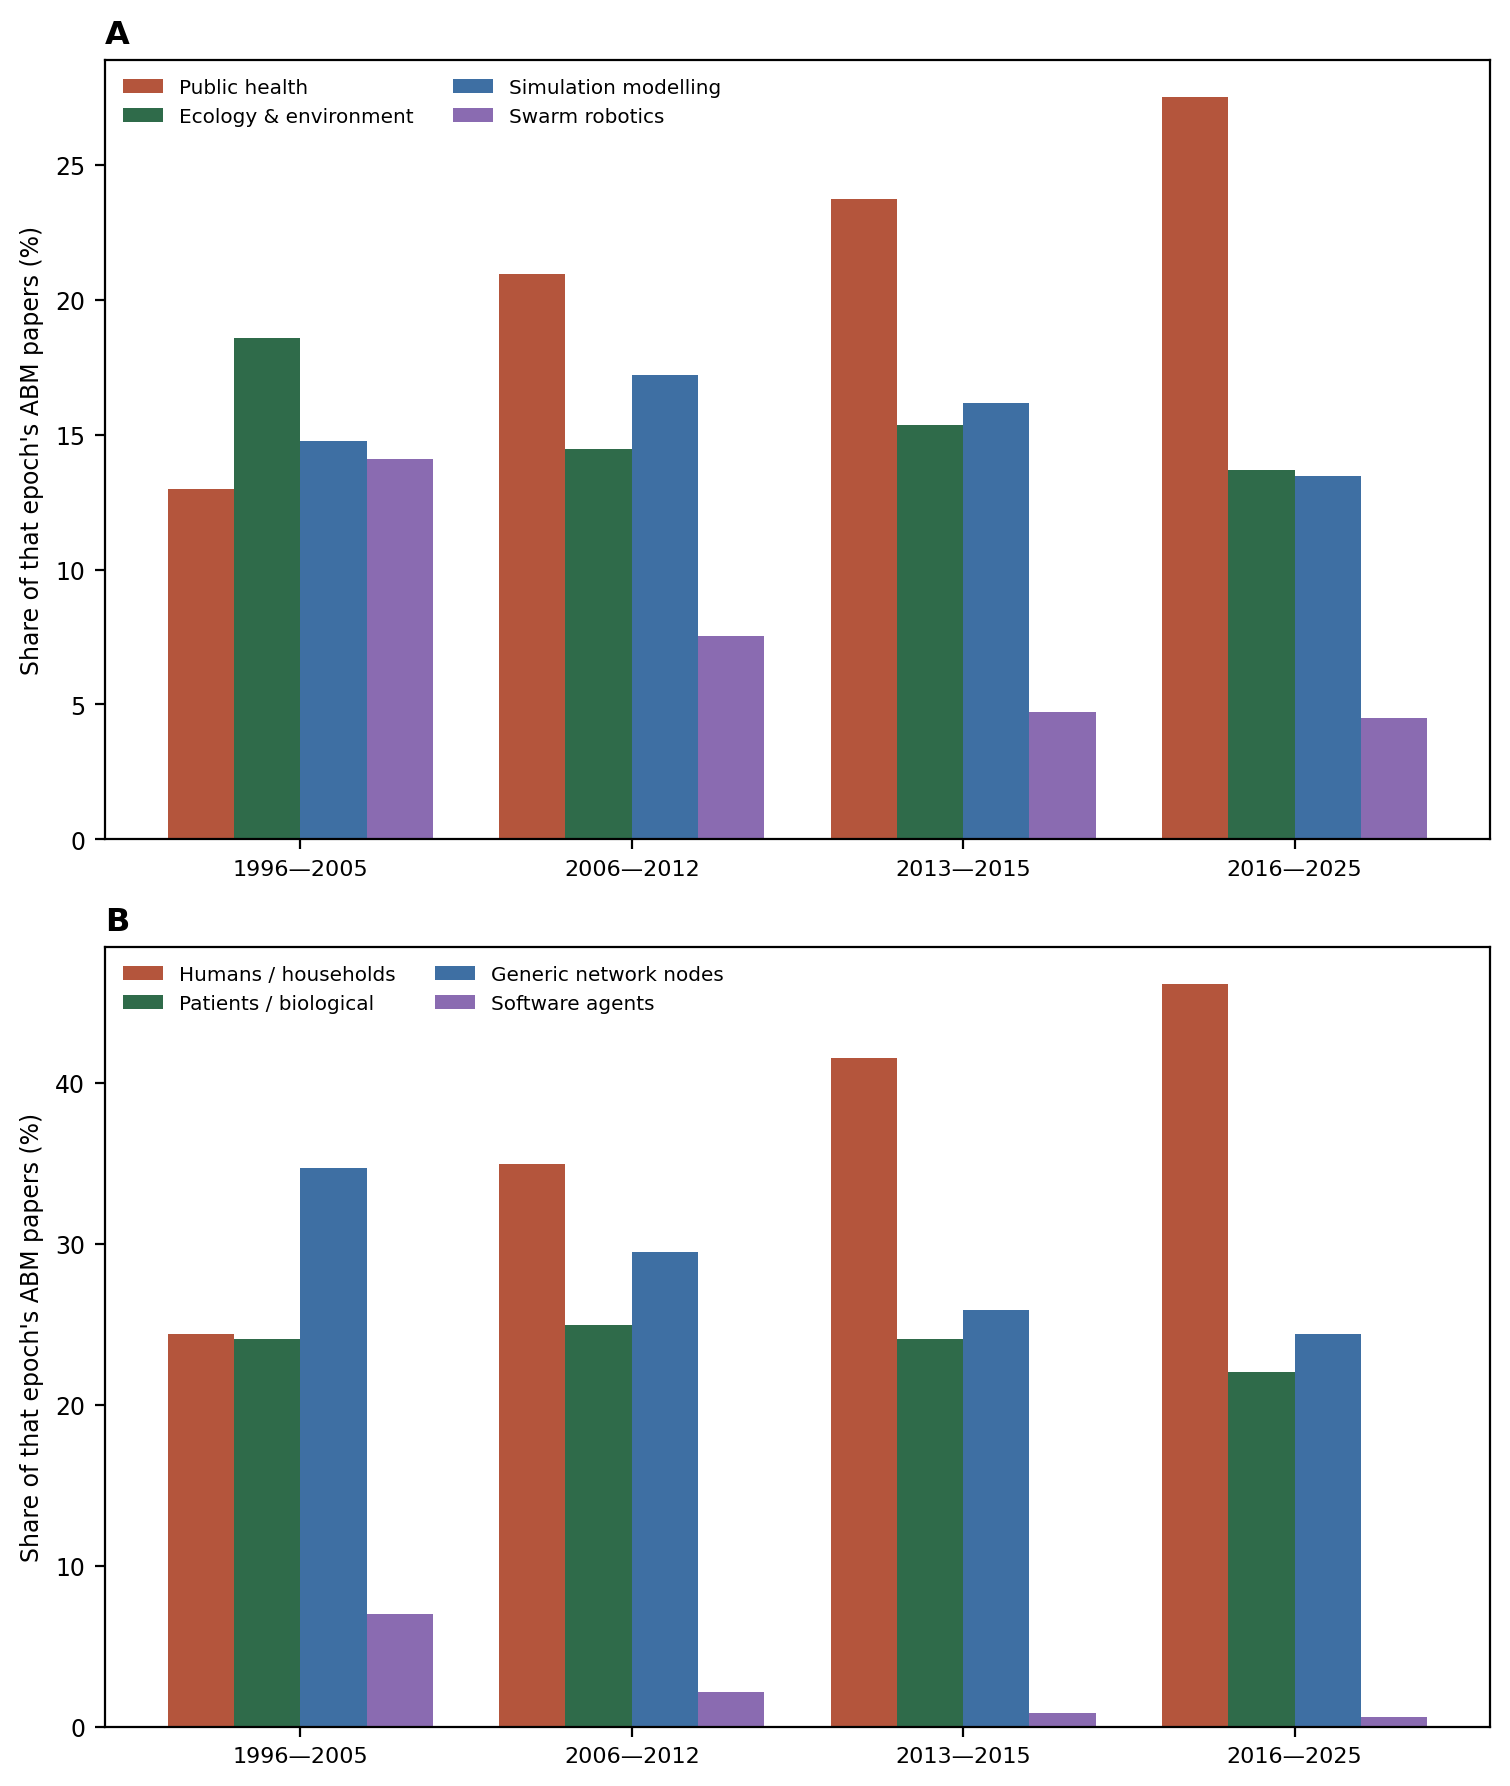
\includegraphics[width=0.88\textwidth,height=0.78\textheight,keepaspectratio]{figures/figure_20.png}
\setcounter{figure}{21}
\caption{Temporal evolution of research topics and modeled agent types.}
\label{fig:figure22}
\end{figure}

These changes are best understood as interdependent rather than sequential. Broader applications create demand for richer behavioral mechanisms; richer mechanisms heighten the need for empirical validation and shared standards; and the collaboration network shapes how those standards spread. The central question is therefore not whether LLMs will replace conventional ABM, but whether the field can incorporate generative decision mechanisms without sacrificing transparency, calibration, and reproducibility.

This synthesis yields five priorities. First, evaluate behavior against empirical benchmarks rather than conversational plausibility alone. Second, report the LLM’s function and position in the model, distinguishing internal decision mechanisms from supporting uses. Third, extend ODD-style reporting to include prompts, model versions, seeds, memory, retrieval, and safeguards. Fourth, develop cross-domain benchmarks that connect epidemiology, mobility, social influence, and policy models. Fifth, examine collaboration networks as channels of methodological diffusion, including whether LLM-enabled papers bridge existing groups or form a weakly connected cluster.

\begin{figure}[htbp]
\centering
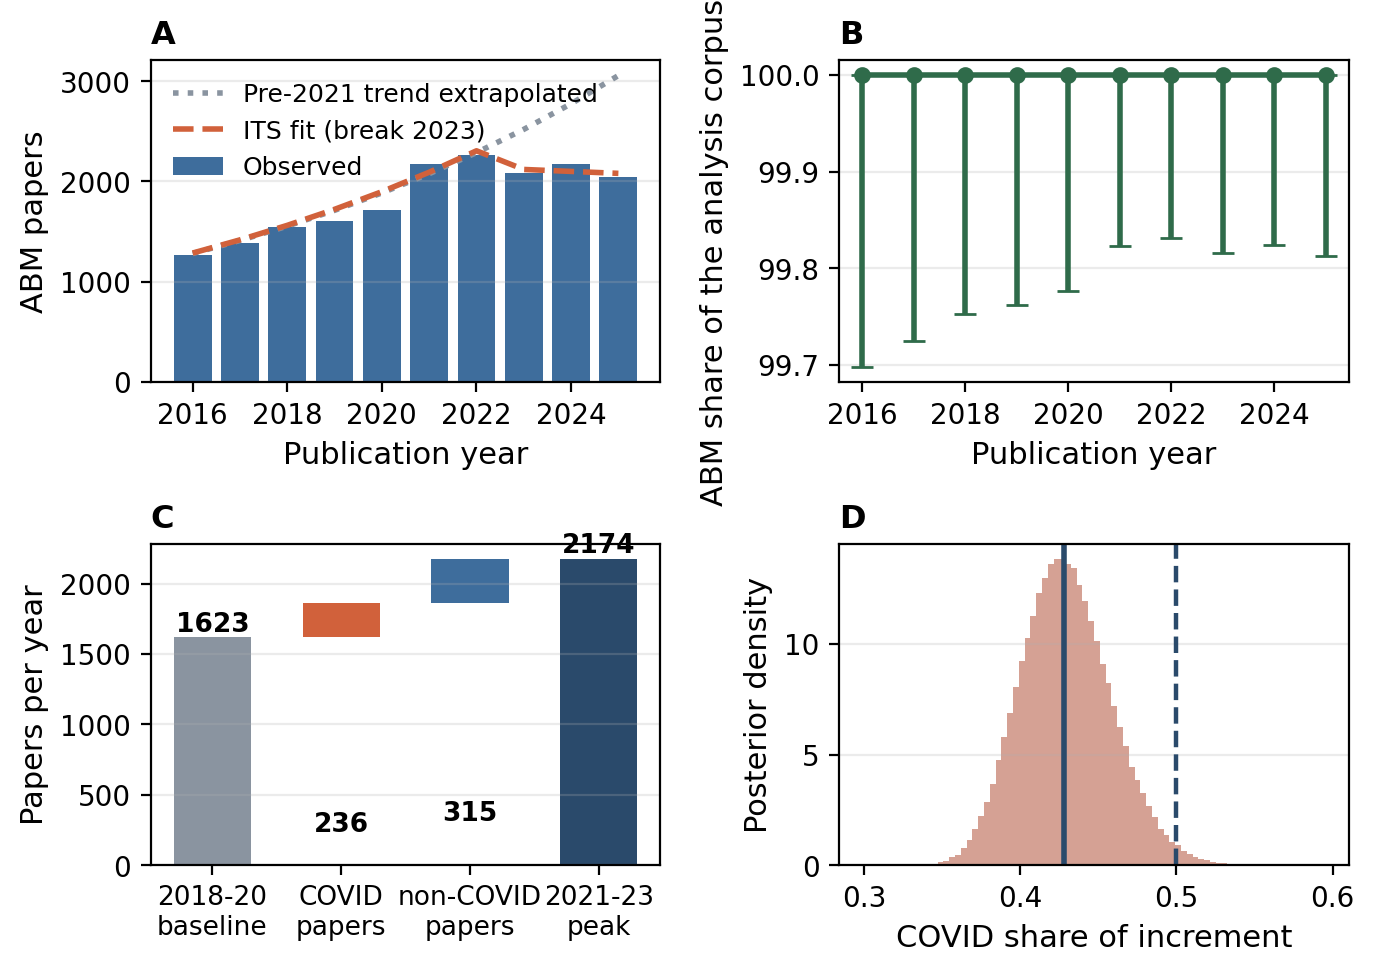
\includegraphics[width=0.88\textwidth,height=0.78\textheight,keepaspectratio]{figures/figure_21.png}
\setcounter{figure}{22}
\caption{Statistical examination of the 2021–2023 publication peak: breakpoint, ABM share, decomposition, and posterior distribution.}
\label{fig:figure23}
\end{figure}
\section{Conclusion}

ABM is in a period of sustained expansion, broad application, human-centered modeling, and increasingly international collaboration. The corpus shows that LLM adoption is rising but remains at an early stage: most ABM papers are not LLM-enabled, and current use is concentrated in a limited set of behavioral and decision functions. Meanwhile, collaboration networks are becoming more modular, making interoperability across specialized communities an important condition for future progress. The field’s next advance will not be measured by adoption alone, but by whether generative agents can be empirically validated, theoretically interpreted, computationally reproduced, and compared across research communities.

\section*{References}
\bibliographystyle{apalike}
\nocite{*}
\bibliography{references}
\end{document}
